
% Default to the notebook output style

    


% Inherit from the specified cell style.




    
\documentclass[11pt]{article}

    
    
    \usepackage[T1]{fontenc}
    % Nicer default font (+ math font) than Computer Modern for most use cases
    \usepackage{mathpazo}

    % Basic figure setup, for now with no caption control since it's done
    % automatically by Pandoc (which extracts ![](path) syntax from Markdown).
    \usepackage{graphicx}
    % We will generate all images so they have a width \maxwidth. This means
    % that they will get their normal width if they fit onto the page, but
    % are scaled down if they would overflow the margins.
    \makeatletter
    \def\maxwidth{\ifdim\Gin@nat@width>\linewidth\linewidth
    \else\Gin@nat@width\fi}
    \makeatother
    \let\Oldincludegraphics\includegraphics
    % Set max figure width to be 80% of text width, for now hardcoded.
    \renewcommand{\includegraphics}[1]{\Oldincludegraphics[width=.8\maxwidth]{#1}}
    % Ensure that by default, figures have no caption (until we provide a
    % proper Figure object with a Caption API and a way to capture that
    % in the conversion process - todo).
    \usepackage{caption}
    \DeclareCaptionLabelFormat{nolabel}{}
    \captionsetup{labelformat=nolabel}

    \usepackage{adjustbox} % Used to constrain images to a maximum size 
    \usepackage{xcolor} % Allow colors to be defined
    \usepackage{enumerate} % Needed for markdown enumerations to work
    \usepackage{geometry} % Used to adjust the document margins
    \usepackage{amsmath} % Equations
    \usepackage{amssymb} % Equations
    \usepackage{textcomp} % defines textquotesingle
    % Hack from http://tex.stackexchange.com/a/47451/13684:
    \AtBeginDocument{%
        \def\PYZsq{\textquotesingle}% Upright quotes in Pygmentized code
    }
    \usepackage{upquote} % Upright quotes for verbatim code
    \usepackage{eurosym} % defines \euro
    \usepackage[mathletters]{ucs} % Extended unicode (utf-8) support
    \usepackage[utf8x]{inputenc} % Allow utf-8 characters in the tex document
    \usepackage{fancyvrb} % verbatim replacement that allows latex
    \usepackage{grffile} % extends the file name processing of package graphics 
                         % to support a larger range 
    % The hyperref package gives us a pdf with properly built
    % internal navigation ('pdf bookmarks' for the table of contents,
    % internal cross-reference links, web links for URLs, etc.)
    \usepackage{hyperref}
    \usepackage{longtable} % longtable support required by pandoc >1.10
    \usepackage{booktabs}  % table support for pandoc > 1.12.2
    \usepackage[inline]{enumitem} % IRkernel/repr support (it uses the enumerate* environment)
    \usepackage[normalem]{ulem} % ulem is needed to support strikethroughs (\sout)
                                % normalem makes italics be italics, not underlines
    

    
    
    % Colors for the hyperref package
    \definecolor{urlcolor}{rgb}{0,.145,.698}
    \definecolor{linkcolor}{rgb}{.71,0.21,0.01}
    \definecolor{citecolor}{rgb}{.12,.54,.11}

    % ANSI colors
    \definecolor{ansi-black}{HTML}{3E424D}
    \definecolor{ansi-black-intense}{HTML}{282C36}
    \definecolor{ansi-red}{HTML}{E75C58}
    \definecolor{ansi-red-intense}{HTML}{B22B31}
    \definecolor{ansi-green}{HTML}{00A250}
    \definecolor{ansi-green-intense}{HTML}{007427}
    \definecolor{ansi-yellow}{HTML}{DDB62B}
    \definecolor{ansi-yellow-intense}{HTML}{B27D12}
    \definecolor{ansi-blue}{HTML}{208FFB}
    \definecolor{ansi-blue-intense}{HTML}{0065CA}
    \definecolor{ansi-magenta}{HTML}{D160C4}
    \definecolor{ansi-magenta-intense}{HTML}{A03196}
    \definecolor{ansi-cyan}{HTML}{60C6C8}
    \definecolor{ansi-cyan-intense}{HTML}{258F8F}
    \definecolor{ansi-white}{HTML}{C5C1B4}
    \definecolor{ansi-white-intense}{HTML}{A1A6B2}

    % commands and environments needed by pandoc snippets
    % extracted from the output of `pandoc -s`
    \providecommand{\tightlist}{%
      \setlength{\itemsep}{0pt}\setlength{\parskip}{0pt}}
    \DefineVerbatimEnvironment{Highlighting}{Verbatim}{commandchars=\\\{\}}
    % Add ',fontsize=\small' for more characters per line
    \newenvironment{Shaded}{}{}
    \newcommand{\KeywordTok}[1]{\textcolor[rgb]{0.00,0.44,0.13}{\textbf{{#1}}}}
    \newcommand{\DataTypeTok}[1]{\textcolor[rgb]{0.56,0.13,0.00}{{#1}}}
    \newcommand{\DecValTok}[1]{\textcolor[rgb]{0.25,0.63,0.44}{{#1}}}
    \newcommand{\BaseNTok}[1]{\textcolor[rgb]{0.25,0.63,0.44}{{#1}}}
    \newcommand{\FloatTok}[1]{\textcolor[rgb]{0.25,0.63,0.44}{{#1}}}
    \newcommand{\CharTok}[1]{\textcolor[rgb]{0.25,0.44,0.63}{{#1}}}
    \newcommand{\StringTok}[1]{\textcolor[rgb]{0.25,0.44,0.63}{{#1}}}
    \newcommand{\CommentTok}[1]{\textcolor[rgb]{0.38,0.63,0.69}{\textit{{#1}}}}
    \newcommand{\OtherTok}[1]{\textcolor[rgb]{0.00,0.44,0.13}{{#1}}}
    \newcommand{\AlertTok}[1]{\textcolor[rgb]{1.00,0.00,0.00}{\textbf{{#1}}}}
    \newcommand{\FunctionTok}[1]{\textcolor[rgb]{0.02,0.16,0.49}{{#1}}}
    \newcommand{\RegionMarkerTok}[1]{{#1}}
    \newcommand{\ErrorTok}[1]{\textcolor[rgb]{1.00,0.00,0.00}{\textbf{{#1}}}}
    \newcommand{\NormalTok}[1]{{#1}}
    
    % Additional commands for more recent versions of Pandoc
    \newcommand{\ConstantTok}[1]{\textcolor[rgb]{0.53,0.00,0.00}{{#1}}}
    \newcommand{\SpecialCharTok}[1]{\textcolor[rgb]{0.25,0.44,0.63}{{#1}}}
    \newcommand{\VerbatimStringTok}[1]{\textcolor[rgb]{0.25,0.44,0.63}{{#1}}}
    \newcommand{\SpecialStringTok}[1]{\textcolor[rgb]{0.73,0.40,0.53}{{#1}}}
    \newcommand{\ImportTok}[1]{{#1}}
    \newcommand{\DocumentationTok}[1]{\textcolor[rgb]{0.73,0.13,0.13}{\textit{{#1}}}}
    \newcommand{\AnnotationTok}[1]{\textcolor[rgb]{0.38,0.63,0.69}{\textbf{\textit{{#1}}}}}
    \newcommand{\CommentVarTok}[1]{\textcolor[rgb]{0.38,0.63,0.69}{\textbf{\textit{{#1}}}}}
    \newcommand{\VariableTok}[1]{\textcolor[rgb]{0.10,0.09,0.49}{{#1}}}
    \newcommand{\ControlFlowTok}[1]{\textcolor[rgb]{0.00,0.44,0.13}{\textbf{{#1}}}}
    \newcommand{\OperatorTok}[1]{\textcolor[rgb]{0.40,0.40,0.40}{{#1}}}
    \newcommand{\BuiltInTok}[1]{{#1}}
    \newcommand{\ExtensionTok}[1]{{#1}}
    \newcommand{\PreprocessorTok}[1]{\textcolor[rgb]{0.74,0.48,0.00}{{#1}}}
    \newcommand{\AttributeTok}[1]{\textcolor[rgb]{0.49,0.56,0.16}{{#1}}}
    \newcommand{\InformationTok}[1]{\textcolor[rgb]{0.38,0.63,0.69}{\textbf{\textit{{#1}}}}}
    \newcommand{\WarningTok}[1]{\textcolor[rgb]{0.38,0.63,0.69}{\textbf{\textit{{#1}}}}}
    
    
    % Define a nice break command that doesn't care if a line doesn't already
    % exist.
    \def\br{\hspace*{\fill} \\* }
    % Math Jax compatability definitions
    \def\gt{>}
    \def\lt{<}
    % Document parameters
    \title{pr2\_e}
    
    
    

    % Pygments definitions
    
\makeatletter
\def\PY@reset{\let\PY@it=\relax \let\PY@bf=\relax%
    \let\PY@ul=\relax \let\PY@tc=\relax%
    \let\PY@bc=\relax \let\PY@ff=\relax}
\def\PY@tok#1{\csname PY@tok@#1\endcsname}
\def\PY@toks#1+{\ifx\relax#1\empty\else%
    \PY@tok{#1}\expandafter\PY@toks\fi}
\def\PY@do#1{\PY@bc{\PY@tc{\PY@ul{%
    \PY@it{\PY@bf{\PY@ff{#1}}}}}}}
\def\PY#1#2{\PY@reset\PY@toks#1+\relax+\PY@do{#2}}

\expandafter\def\csname PY@tok@w\endcsname{\def\PY@tc##1{\textcolor[rgb]{0.73,0.73,0.73}{##1}}}
\expandafter\def\csname PY@tok@c\endcsname{\let\PY@it=\textit\def\PY@tc##1{\textcolor[rgb]{0.25,0.50,0.50}{##1}}}
\expandafter\def\csname PY@tok@cp\endcsname{\def\PY@tc##1{\textcolor[rgb]{0.74,0.48,0.00}{##1}}}
\expandafter\def\csname PY@tok@k\endcsname{\let\PY@bf=\textbf\def\PY@tc##1{\textcolor[rgb]{0.00,0.50,0.00}{##1}}}
\expandafter\def\csname PY@tok@kp\endcsname{\def\PY@tc##1{\textcolor[rgb]{0.00,0.50,0.00}{##1}}}
\expandafter\def\csname PY@tok@kt\endcsname{\def\PY@tc##1{\textcolor[rgb]{0.69,0.00,0.25}{##1}}}
\expandafter\def\csname PY@tok@o\endcsname{\def\PY@tc##1{\textcolor[rgb]{0.40,0.40,0.40}{##1}}}
\expandafter\def\csname PY@tok@ow\endcsname{\let\PY@bf=\textbf\def\PY@tc##1{\textcolor[rgb]{0.67,0.13,1.00}{##1}}}
\expandafter\def\csname PY@tok@nb\endcsname{\def\PY@tc##1{\textcolor[rgb]{0.00,0.50,0.00}{##1}}}
\expandafter\def\csname PY@tok@nf\endcsname{\def\PY@tc##1{\textcolor[rgb]{0.00,0.00,1.00}{##1}}}
\expandafter\def\csname PY@tok@nc\endcsname{\let\PY@bf=\textbf\def\PY@tc##1{\textcolor[rgb]{0.00,0.00,1.00}{##1}}}
\expandafter\def\csname PY@tok@nn\endcsname{\let\PY@bf=\textbf\def\PY@tc##1{\textcolor[rgb]{0.00,0.00,1.00}{##1}}}
\expandafter\def\csname PY@tok@ne\endcsname{\let\PY@bf=\textbf\def\PY@tc##1{\textcolor[rgb]{0.82,0.25,0.23}{##1}}}
\expandafter\def\csname PY@tok@nv\endcsname{\def\PY@tc##1{\textcolor[rgb]{0.10,0.09,0.49}{##1}}}
\expandafter\def\csname PY@tok@no\endcsname{\def\PY@tc##1{\textcolor[rgb]{0.53,0.00,0.00}{##1}}}
\expandafter\def\csname PY@tok@nl\endcsname{\def\PY@tc##1{\textcolor[rgb]{0.63,0.63,0.00}{##1}}}
\expandafter\def\csname PY@tok@ni\endcsname{\let\PY@bf=\textbf\def\PY@tc##1{\textcolor[rgb]{0.60,0.60,0.60}{##1}}}
\expandafter\def\csname PY@tok@na\endcsname{\def\PY@tc##1{\textcolor[rgb]{0.49,0.56,0.16}{##1}}}
\expandafter\def\csname PY@tok@nt\endcsname{\let\PY@bf=\textbf\def\PY@tc##1{\textcolor[rgb]{0.00,0.50,0.00}{##1}}}
\expandafter\def\csname PY@tok@nd\endcsname{\def\PY@tc##1{\textcolor[rgb]{0.67,0.13,1.00}{##1}}}
\expandafter\def\csname PY@tok@s\endcsname{\def\PY@tc##1{\textcolor[rgb]{0.73,0.13,0.13}{##1}}}
\expandafter\def\csname PY@tok@sd\endcsname{\let\PY@it=\textit\def\PY@tc##1{\textcolor[rgb]{0.73,0.13,0.13}{##1}}}
\expandafter\def\csname PY@tok@si\endcsname{\let\PY@bf=\textbf\def\PY@tc##1{\textcolor[rgb]{0.73,0.40,0.53}{##1}}}
\expandafter\def\csname PY@tok@se\endcsname{\let\PY@bf=\textbf\def\PY@tc##1{\textcolor[rgb]{0.73,0.40,0.13}{##1}}}
\expandafter\def\csname PY@tok@sr\endcsname{\def\PY@tc##1{\textcolor[rgb]{0.73,0.40,0.53}{##1}}}
\expandafter\def\csname PY@tok@ss\endcsname{\def\PY@tc##1{\textcolor[rgb]{0.10,0.09,0.49}{##1}}}
\expandafter\def\csname PY@tok@sx\endcsname{\def\PY@tc##1{\textcolor[rgb]{0.00,0.50,0.00}{##1}}}
\expandafter\def\csname PY@tok@m\endcsname{\def\PY@tc##1{\textcolor[rgb]{0.40,0.40,0.40}{##1}}}
\expandafter\def\csname PY@tok@gh\endcsname{\let\PY@bf=\textbf\def\PY@tc##1{\textcolor[rgb]{0.00,0.00,0.50}{##1}}}
\expandafter\def\csname PY@tok@gu\endcsname{\let\PY@bf=\textbf\def\PY@tc##1{\textcolor[rgb]{0.50,0.00,0.50}{##1}}}
\expandafter\def\csname PY@tok@gd\endcsname{\def\PY@tc##1{\textcolor[rgb]{0.63,0.00,0.00}{##1}}}
\expandafter\def\csname PY@tok@gi\endcsname{\def\PY@tc##1{\textcolor[rgb]{0.00,0.63,0.00}{##1}}}
\expandafter\def\csname PY@tok@gr\endcsname{\def\PY@tc##1{\textcolor[rgb]{1.00,0.00,0.00}{##1}}}
\expandafter\def\csname PY@tok@ge\endcsname{\let\PY@it=\textit}
\expandafter\def\csname PY@tok@gs\endcsname{\let\PY@bf=\textbf}
\expandafter\def\csname PY@tok@gp\endcsname{\let\PY@bf=\textbf\def\PY@tc##1{\textcolor[rgb]{0.00,0.00,0.50}{##1}}}
\expandafter\def\csname PY@tok@go\endcsname{\def\PY@tc##1{\textcolor[rgb]{0.53,0.53,0.53}{##1}}}
\expandafter\def\csname PY@tok@gt\endcsname{\def\PY@tc##1{\textcolor[rgb]{0.00,0.27,0.87}{##1}}}
\expandafter\def\csname PY@tok@err\endcsname{\def\PY@bc##1{\setlength{\fboxsep}{0pt}\fcolorbox[rgb]{1.00,0.00,0.00}{1,1,1}{\strut ##1}}}
\expandafter\def\csname PY@tok@kc\endcsname{\let\PY@bf=\textbf\def\PY@tc##1{\textcolor[rgb]{0.00,0.50,0.00}{##1}}}
\expandafter\def\csname PY@tok@kd\endcsname{\let\PY@bf=\textbf\def\PY@tc##1{\textcolor[rgb]{0.00,0.50,0.00}{##1}}}
\expandafter\def\csname PY@tok@kn\endcsname{\let\PY@bf=\textbf\def\PY@tc##1{\textcolor[rgb]{0.00,0.50,0.00}{##1}}}
\expandafter\def\csname PY@tok@kr\endcsname{\let\PY@bf=\textbf\def\PY@tc##1{\textcolor[rgb]{0.00,0.50,0.00}{##1}}}
\expandafter\def\csname PY@tok@bp\endcsname{\def\PY@tc##1{\textcolor[rgb]{0.00,0.50,0.00}{##1}}}
\expandafter\def\csname PY@tok@fm\endcsname{\def\PY@tc##1{\textcolor[rgb]{0.00,0.00,1.00}{##1}}}
\expandafter\def\csname PY@tok@vc\endcsname{\def\PY@tc##1{\textcolor[rgb]{0.10,0.09,0.49}{##1}}}
\expandafter\def\csname PY@tok@vg\endcsname{\def\PY@tc##1{\textcolor[rgb]{0.10,0.09,0.49}{##1}}}
\expandafter\def\csname PY@tok@vi\endcsname{\def\PY@tc##1{\textcolor[rgb]{0.10,0.09,0.49}{##1}}}
\expandafter\def\csname PY@tok@vm\endcsname{\def\PY@tc##1{\textcolor[rgb]{0.10,0.09,0.49}{##1}}}
\expandafter\def\csname PY@tok@sa\endcsname{\def\PY@tc##1{\textcolor[rgb]{0.73,0.13,0.13}{##1}}}
\expandafter\def\csname PY@tok@sb\endcsname{\def\PY@tc##1{\textcolor[rgb]{0.73,0.13,0.13}{##1}}}
\expandafter\def\csname PY@tok@sc\endcsname{\def\PY@tc##1{\textcolor[rgb]{0.73,0.13,0.13}{##1}}}
\expandafter\def\csname PY@tok@dl\endcsname{\def\PY@tc##1{\textcolor[rgb]{0.73,0.13,0.13}{##1}}}
\expandafter\def\csname PY@tok@s2\endcsname{\def\PY@tc##1{\textcolor[rgb]{0.73,0.13,0.13}{##1}}}
\expandafter\def\csname PY@tok@sh\endcsname{\def\PY@tc##1{\textcolor[rgb]{0.73,0.13,0.13}{##1}}}
\expandafter\def\csname PY@tok@s1\endcsname{\def\PY@tc##1{\textcolor[rgb]{0.73,0.13,0.13}{##1}}}
\expandafter\def\csname PY@tok@mb\endcsname{\def\PY@tc##1{\textcolor[rgb]{0.40,0.40,0.40}{##1}}}
\expandafter\def\csname PY@tok@mf\endcsname{\def\PY@tc##1{\textcolor[rgb]{0.40,0.40,0.40}{##1}}}
\expandafter\def\csname PY@tok@mh\endcsname{\def\PY@tc##1{\textcolor[rgb]{0.40,0.40,0.40}{##1}}}
\expandafter\def\csname PY@tok@mi\endcsname{\def\PY@tc##1{\textcolor[rgb]{0.40,0.40,0.40}{##1}}}
\expandafter\def\csname PY@tok@il\endcsname{\def\PY@tc##1{\textcolor[rgb]{0.40,0.40,0.40}{##1}}}
\expandafter\def\csname PY@tok@mo\endcsname{\def\PY@tc##1{\textcolor[rgb]{0.40,0.40,0.40}{##1}}}
\expandafter\def\csname PY@tok@ch\endcsname{\let\PY@it=\textit\def\PY@tc##1{\textcolor[rgb]{0.25,0.50,0.50}{##1}}}
\expandafter\def\csname PY@tok@cm\endcsname{\let\PY@it=\textit\def\PY@tc##1{\textcolor[rgb]{0.25,0.50,0.50}{##1}}}
\expandafter\def\csname PY@tok@cpf\endcsname{\let\PY@it=\textit\def\PY@tc##1{\textcolor[rgb]{0.25,0.50,0.50}{##1}}}
\expandafter\def\csname PY@tok@c1\endcsname{\let\PY@it=\textit\def\PY@tc##1{\textcolor[rgb]{0.25,0.50,0.50}{##1}}}
\expandafter\def\csname PY@tok@cs\endcsname{\let\PY@it=\textit\def\PY@tc##1{\textcolor[rgb]{0.25,0.50,0.50}{##1}}}

\def\PYZbs{\char`\\}
\def\PYZus{\char`\_}
\def\PYZob{\char`\{}
\def\PYZcb{\char`\}}
\def\PYZca{\char`\^}
\def\PYZam{\char`\&}
\def\PYZlt{\char`\<}
\def\PYZgt{\char`\>}
\def\PYZsh{\char`\#}
\def\PYZpc{\char`\%}
\def\PYZdl{\char`\$}
\def\PYZhy{\char`\-}
\def\PYZsq{\char`\'}
\def\PYZdq{\char`\"}
\def\PYZti{\char`\~}
% for compatibility with earlier versions
\def\PYZat{@}
\def\PYZlb{[}
\def\PYZrb{]}
\makeatother


    % Exact colors from NB
    \definecolor{incolor}{rgb}{0.0, 0.0, 0.5}
    \definecolor{outcolor}{rgb}{0.545, 0.0, 0.0}



    
    % Prevent overflowing lines due to hard-to-break entities
    \sloppy 
    % Setup hyperref package
    \hypersetup{
      breaklinks=true,  % so long urls are correctly broken across lines
      colorlinks=true,
      urlcolor=urlcolor,
      linkcolor=linkcolor,
      citecolor=citecolor,
      }
    % Slightly bigger margins than the latex defaults
    
    \geometry{verbose,tmargin=1in,bmargin=1in,lmargin=1in,rmargin=1in}
    
    

    \begin{document}
    
    
    \maketitle
    
    

    
    \section{Práctica Métodos de Simulación - Parte
2}\label{pruxe1ctica-muxe9todos-de-simulaciuxf3n---parte-2}

    \subsection{Elena Rivas, Teresa Grau, Ignacio
Casso}\label{elena-rivas-teresa-grau-ignacio-casso}

    \textbf{Enunciado. Simulación de sucesos discretos.}

Un taller de fabricación se dedica a procesar tres tipos de piezas, para
ello el taller consta de cuatro células de procesamiento.

En el interior de cada célula se dispone de una máquina de procesado,
excepto en la célula 3 formada por dos máquinas con las mismas
características, y de un almacén (de capacidad ilimitada).

La secuencia de fabricación de cada una de las piezas así como los
tiempos de procesado (expresados en minutos y distribuidos según una
triangular) en cada célula se muestran en la siguiente tabla:

\begin{figure}
\centering
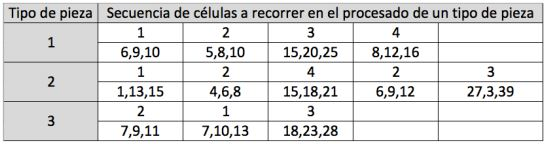
\includegraphics{./imagenes/Captura_tabla_ms.JPG}
\caption{Captura\_tabla\_ms.JPG}
\end{figure}

Los tiempos entre llegadas de las piezas al taller tiene carácter
aleatorio. En el fichero \texttt{llegadas.txt} se proporciona una
muestra de tiempos entre llegadas de piezas. Contrástese si la
distribución de dichos tiempos es normal (truncada), weibull o
exponencial y estímense los parámetros de la distribución
correspondiente.

El fichero \texttt{piezas.txt} incluye un histórico de piezas que han
llegado al taller, que nos permitirá identificar la proporción de piezas
que hay de cada uno de los tres tipos.

Los tiempos de transporte de cada pieza entre las diferentes células es
de 2 minutos.

A. Suponiendo que el taller trabaja de forma ininterrumpida (hay tres
turnos de trabajadores), simular el comportamiento del sistema durante 2
meses para estimar el tiempo mínimo, medio y máximo que tardan en
fabricarse los tres tipos de piezas, el número medio de piezas esperando
en cada una de las 4 células y la proporción de tiempo que están ociosas
las máquinas de procesado de las células.

B. Calcular las medidas anteriores si el tiempo de transporte de las
piezas entre las distintas células se reduce la mitad.

En caso de que fuese posible disponer de una máquina de procesado
adicional, ¿en qué célula sería más beneficioso ponerla?

    \subsection{Distribución de los tiempos de
llegada}\label{distribuciuxf3n-de-los-tiempos-de-llegada}

    En primer lugar comprobamos si los tiempos de llegada proporcionados en
el fichero \texttt{E1.llegadas.txt} siguen una distribución normal
truncada, weibull o exponencial, y estimar los parámetros
correspondientes. Para ello podemos usar los contrastes de hipótesis
vistos en clase, en concreto el contraste de
\textbf{\emph{Kolmogorov-Smirnov}}.

    En estadística, la prueba de \emph{Kolmogórov-Smirnov} (también prueba
K-S) es una prueba no paramétrica que determina la bondad de ajuste de
dos distribuciones de probabilidad entre sí. Consiste en lo siguiente:

    Deseamos contrastar la hipotesis \[H_0: F_n(x) = F_0(x)\]

Para ello, utilizamos el estadístico de contraste
\[D = sup|\hat F_n(x_i) - F_0(x_i)|\] donde: * \(x_i\) es el i-ésimo
valor observado en la muestra (cuyos valores se han ordenado previamente
de menor a mayor). * \(\hat F_n(x_i)\) es un estimador de la
probabilidad de observar valores menores o iguales que \(x_i\). *
\(F_0(x_i)\) es la probabilidad de observar valores menores o iguales
que \(x_i\) cuando \(H_0\) es cierta.

Así pues, \(D\) es la mayor diferencia absoluta observada entre la
frecuencia acumulada observada \(\hat F_n(x_i)\) y la frecuencia
acumulada teórica \(F_0(x_i)\), obtenida a partir de la distribución de
probabilidad que se especifica como hipótesis nula.

Si los valores observados \(\hat F_n(x_i)\) son similares a los
esperados \(F_0(x_i)\), el valor de \(D\) será pequeño. Cuanto mayor sea
la discrepancia entre la distribución empírica \(\hat F_n(x_i)\) y la
distribución teórica \(F_0(x_i)\), mayor será el valor de \(D\).

    \begin{Verbatim}[commandchars=\\\{\}]
{\color{incolor}In [{\color{incolor}1}]:} \PY{k+kn}{import} \PY{n+nn}{numpy} \PY{k}{as} \PY{n+nn}{np}
        \PY{k+kn}{import} \PY{n+nn}{random}
        \PY{k+kn}{import} \PY{n+nn}{queue}
        \PY{k+kn}{import} \PY{n+nn}{math}
        \PY{k+kn}{import} \PY{n+nn}{matplotlib}\PY{n+nn}{.}\PY{n+nn}{pyplot} \PY{k}{as} \PY{n+nn}{plt}
        \PY{k+kn}{from} \PY{n+nn}{scipy} \PY{k}{import} \PY{n}{stats}
        \PY{k+kn}{from} \PY{n+nn}{scipy}\PY{n+nn}{.}\PY{n+nn}{stats} \PY{k}{import} \PY{n}{kstest}
\end{Verbatim}


    \begin{Verbatim}[commandchars=\\\{\}]
{\color{incolor}In [{\color{incolor}2}]:} \PY{n}{archivo\PYZus{}llegadas} \PY{o}{=} \PY{n+nb}{open}\PY{p}{(}\PY{l+s+s1}{\PYZsq{}}\PY{l+s+s1}{./E1.llegadas.txt}\PY{l+s+s1}{\PYZsq{}}\PY{p}{,} \PY{l+s+s1}{\PYZsq{}}\PY{l+s+s1}{r}\PY{l+s+s1}{\PYZsq{}}\PY{p}{)}
        \PY{n}{llegadas} \PY{o}{=} \PY{p}{[}\PY{n+nb}{float}\PY{p}{(}\PY{n}{line}\PY{p}{)} \PY{k}{for} \PY{n}{line} \PY{o+ow}{in} \PY{n}{archivo\PYZus{}llegadas}\PY{o}{.}\PY{n}{readlines}\PY{p}{(}\PY{p}{)}\PY{p}{]}
        \PY{n}{archivo\PYZus{}llegadas}\PY{o}{.}\PY{n}{close}\PY{p}{(}\PY{p}{)}
\end{Verbatim}


    \begin{Verbatim}[commandchars=\\\{\}]
{\color{incolor}In [{\color{incolor}3}]:} \PY{n}{archivo\PYZus{}piezas} \PY{o}{=} \PY{n+nb}{open}\PY{p}{(}\PY{l+s+s1}{\PYZsq{}}\PY{l+s+s1}{./E1.piezas.txt}\PY{l+s+s1}{\PYZsq{}}\PY{p}{,} \PY{l+s+s1}{\PYZsq{}}\PY{l+s+s1}{r}\PY{l+s+s1}{\PYZsq{}}\PY{p}{)}
        \PY{n}{piezas} \PY{o}{=} \PY{p}{[}\PY{n+nb}{int}\PY{p}{(}\PY{n}{line}\PY{p}{)} \PY{k}{for} \PY{n}{line} \PY{o+ow}{in} \PY{n}{archivo\PYZus{}piezas}\PY{o}{.}\PY{n}{readlines}\PY{p}{(}\PY{p}{)}\PY{p}{]}
        \PY{n}{archivo\PYZus{}piezas}\PY{o}{.}\PY{n}{close}\PY{p}{(}\PY{p}{)}
\end{Verbatim}


    Con el paquete estadístico \texttt{stats} de la librería \texttt{scipy}
de Python podemos contrastar la distribución de nuestra muestra con la
prueba de \textbf{\emph{Kolmogorov}}.

    \begin{Verbatim}[commandchars=\\\{\}]
{\color{incolor}In [{\color{incolor}4}]:} \PY{k+kn}{from} \PY{n+nn}{scipy}\PY{n+nn}{.}\PY{n+nn}{stats} \PY{k}{import} \PY{n}{expon}\PY{p}{,} \PY{n}{exponweib}\PY{p}{,} \PY{n}{truncnorm}
\end{Verbatim}


    Comenzamos testando la distribución exponencial. Según la documentación
del paquete \texttt{stats}, la función de densidad de la exponencial es:
\[f(x) = \exp(-x)\] para \(x\geq0\).

    La densidad de probabilidad anterior se define en la forma
"estandarizada". Para cambiar y/o escalar la distribución, utilizamos
los parámetros \texttt{loc} y \texttt{scale}. Específicamente,
\texttt{expon.pdf\ (x,\ loc,\ scale)} (probability density function),
que es equivalente a \texttt{expon.pd(y)\ /\ scale} con
\texttt{y\ =\ (x\ -\ loc)\ /\ scale}.

Una parametrización común de la exponencial es en términos del parámetro
\emph{lambda}, tal que \texttt{pdf\ =\ lambda\ *\ exp\ (-lambda\ *\ x)}.
Esta parametrización corresponde a usar \texttt{scale\ =\ 1/lambda}.

Para realizar el contraste con la librería \texttt{stats} primero
necesitamos estimar los parametros que corresponderían a nuestra muestra
para la distribución que queremos contrastar. Para esta tarea,
\texttt{stats} cuenta con el método
\texttt{scipy.stats.rv\_continuous.fit}.

Éste devuelve los \emph{MLE} para los parámetros de forma (si
corresponde), ubicación y escala a partir de la muestra. MLE significa
Estimación de máxima verosimilitud (Maximum Likelihood Estimate). Hay
que tener en cuenta que \texttt{fit} se calcula al maximizar una función
\emph{log-likehood}, aplicando una penalización para muestras fuera del
rango de distribución. No se garantiza que la respuesta devuelta sea el
MLE globalmente óptimo, puede que solo sea óptimo local o la
optimización puede fallar por completo.

Una vez estimados los parametros de la exponencial, ya podemos utilizar
el método \texttt{scipy.stats.kstest} que ejecuta la prueba de
Kolmogorov-Smirnov para comprobar la bondad del ajuste. Que devuelve el
valor del estadístico \(D\) y un \textbf{\emph{p-valor}}.

La decisión de aceptar o rechazar la hipotesis es tomada a partir de
este \textbf{\emph{p-valor}}. Si el \textbf{\emph{p-valor}} es grande
significa que, siendo cierta la hipótesis nula, el valor observado del
estadístico \(D\) era esperable, y por tanto, no hay razón para rechazar
la hipótesis. Asimismo, si el \textbf{\emph{p-valor}} es pequeño, indica
que, siendo cierta la hipótesis nula, es muy difícil que se produjera el
valor de \(D\) que efectivamente se ha observado. Ello obliga a poner
muy en duda, y por tanto a rechazar la hipótesis nula.

    Ya podemos testar la distribución exponencial:

    \begin{Verbatim}[commandchars=\\\{\}]
{\color{incolor}In [{\color{incolor}6}]:} \PY{n}{loc}\PY{p}{,} \PY{n}{scale} \PY{o}{=} \PY{n}{expon}\PY{o}{.}\PY{n}{fit}\PY{p}{(}\PY{n}{llegadas}\PY{p}{)}
        
        \PY{n}{kstest}\PY{p}{(}\PY{n}{llegadas}\PY{p}{,}\PY{l+s+s1}{\PYZsq{}}\PY{l+s+s1}{expon}\PY{l+s+s1}{\PYZsq{}}\PY{p}{,} \PY{p}{(}\PY{n}{loc}\PY{p}{,} \PY{n}{scale}\PY{p}{)}\PY{p}{)}
\end{Verbatim}


\begin{Verbatim}[commandchars=\\\{\}]
{\color{outcolor}Out[{\color{outcolor}6}]:} KstestResult(statistic=0.010470200051473033, pvalue=0.6434208493162717)
\end{Verbatim}
            
    Hipotesis no rechazada. Los párametros serían:

    \begin{Verbatim}[commandchars=\\\{\}]
{\color{incolor}In [{\color{incolor}7}]:} \PY{n+nb}{print}\PY{p}{(}\PY{p}{(}\PY{n}{loc}\PY{p}{,} \PY{n}{scale}\PY{p}{)}\PY{p}{)}
\end{Verbatim}


    \begin{Verbatim}[commandchars=\\\{\}]
(0.001173691, 12.9963028643654)

    \end{Verbatim}

    A continuación testamos la distribución de weibull, que según la
documentación de \texttt{stats} tiene la siguiente funcion de
distribución: \[f(x,a,c) = ac(1-exp(-x^c))^{a-1}exp(-x^c)^{c-1}\] para
\(x>0\), \(a>0\), \(c>0\).

    \(a\) y \(c\) son parámetros de forma. La densidad de probabilidad
anterior se define en la forma "estandarizada". Para cambiar y/o escalar
la distribución, al igual que explicamos antes en la exponencial, se
utilizan los parametros \emph{loc} y \emph{scale}. Concretamente,
\texttt{exponweib.pdf(x,\ a,\ c,\ loc,\ scale)}, que es equivalente a
\texttt{exponweib.pdf(y,\ a,\ c)\ /\ scale} con
\texttt{y\ =\ (x\ -\ loc)\ /\ scale.}

    \begin{Verbatim}[commandchars=\\\{\}]
{\color{incolor}In [{\color{incolor}8}]:} \PY{n}{params} \PY{o}{=} \PY{n}{exponweib}\PY{o}{.}\PY{n}{fit}\PY{p}{(}\PY{n}{llegadas}\PY{p}{,} \PY{n}{fa}\PY{o}{=}\PY{l+m+mi}{1}\PY{p}{)} \PY{c+c1}{\PYZsh{} an exponential weibull with a = 1 is the normal weibull}
        
        \PY{n}{kstest}\PY{p}{(}\PY{n}{llegadas}\PY{p}{,}\PY{l+s+s1}{\PYZsq{}}\PY{l+s+s1}{exponweib}\PY{l+s+s1}{\PYZsq{}}\PY{p}{,} \PY{n}{args}\PY{o}{=}\PY{n}{params}\PY{p}{)}
\end{Verbatim}


\begin{Verbatim}[commandchars=\\\{\}]
{\color{outcolor}Out[{\color{outcolor}8}]:} KstestResult(statistic=0.009058871617199038, pvalue=0.8064767011732374)
\end{Verbatim}
            
    Hypotesis not rejected

    \begin{Verbatim}[commandchars=\\\{\}]
{\color{incolor}In [{\color{incolor}9}]:} \PY{n+nb}{print}\PY{p}{(}\PY{n}{params}\PY{p}{)}
\end{Verbatim}


    \begin{Verbatim}[commandchars=\\\{\}]
(1, 0.9835163304844294, 0.0011736909999999997, 12.917026888061788)

    \end{Verbatim}

    Tampoco rechaza la hipotesis de que nuestra muestra siga una
distribución Weibull. Esto podemos explicarlo observando los parametros
que obtenemos con la funcion \texttt{fit}. Observamos que el parametro
\(c\) es casi 1 (c = 0.98), cuando se da esto lo que en realidad tenemos
es una exponencial. Por eso la hipotesis no es rechazada.

    Y por último testamos la distribución normal truncada:

    \begin{Verbatim}[commandchars=\\\{\}]
{\color{incolor}In [{\color{incolor}5}]:} \PY{k+kn}{from} \PY{n+nn}{scipy}\PY{n+nn}{.}\PY{n+nn}{stats} \PY{k}{import} \PY{n}{truncnorm}
        
        \PY{n}{a}\PY{p}{,}\PY{n}{b}\PY{p}{,}\PY{n}{loc}\PY{p}{,}\PY{n}{scale} \PY{o}{=} \PY{n}{truncnorm}\PY{o}{.}\PY{n}{fit}\PY{p}{(}\PY{n}{llegadas}\PY{p}{)}
        
        \PY{c+c1}{\PYZsh{} The bounds are given w.r.t the standard distribution, prior to applying scale and location paramenters.}
        \PY{c+c1}{\PYZsh{} Therefore we can\PYZsq{}t specify that the lower bound is 0 (fa=0). The information we have is that}
        \PY{c+c1}{\PYZsh{} a = \PYZhy{}loc, but that is a constraint we can not pass to the method fit. To satisfy the constraint, we propose}
        \PY{c+c1}{\PYZsh{} the following fixpoint}
        
        \PY{k}{while} \PY{n+nb}{abs}\PY{p}{(}\PY{n}{loc}\PY{o}{+}\PY{n}{a}\PY{p}{)} \PY{o}{\PYZgt{}} \PY{l+m+mf}{0.0001}\PY{p}{:}
            \PY{n}{a}\PY{p}{,}\PY{n}{b}\PY{p}{,}\PY{n}{loc}\PY{p}{,}\PY{n}{scale} \PY{o}{=} \PY{n}{truncnorm}\PY{o}{.}\PY{n}{fit}\PY{p}{(}\PY{n}{llegadas}\PY{p}{,} \PY{n}{fa}\PY{o}{=}\PY{o}{\PYZhy{}}\PY{n}{loc}\PY{p}{)}
            
        \PY{c+c1}{\PYZsh{} just needs one iteration}
        
        \PY{n}{kstest}\PY{p}{(}\PY{n}{llegadas}\PY{p}{,}\PY{l+s+s1}{\PYZsq{}}\PY{l+s+s1}{truncnorm}\PY{l+s+s1}{\PYZsq{}}\PY{p}{,} \PY{p}{(}\PY{n}{a}\PY{p}{,}\PY{n}{b}\PY{p}{,}\PY{n}{loc}\PY{p}{,}\PY{n}{scale}\PY{p}{)}\PY{p}{)}
\end{Verbatim}


    \begin{Verbatim}[commandchars=\\\{\}]
/usr/lib/python3/dist-packages/scipy/stats/\_continuous\_distns.py:4846: RuntimeWarning: divide by zero encountered in log
  self.\_logdelta = np.log(self.\_delta)
/usr/lib/python3/dist-packages/scipy/stats/\_continuous\_distns.py:4846: RuntimeWarning: invalid value encountered in log
  self.\_logdelta = np.log(self.\_delta)

    \end{Verbatim}

\begin{Verbatim}[commandchars=\\\{\}]
{\color{outcolor}Out[{\color{outcolor}5}]:} KstestResult(statistic=0.16126924639176748, pvalue=2.2424395794550417e-113)
\end{Verbatim}
            
    La hipotesis es rechazada. Por tanto, nuestra muestra sigue una
distribución exponencial con los siguientes parametros \texttt{loc} y
\texttt{scale}:

    \begin{Verbatim}[commandchars=\\\{\}]
{\color{incolor}In [{\color{incolor}11}]:} \PY{n}{loc}\PY{p}{,} \PY{n}{scale} \PY{o}{=} \PY{n}{expon}\PY{o}{.}\PY{n}{fit}\PY{p}{(}\PY{n}{llegadas}\PY{p}{)}
         \PY{n+nb}{print}\PY{p}{(}\PY{p}{(}\PY{n}{loc}\PY{p}{,} \PY{n}{scale}\PY{p}{)}\PY{p}{)}
\end{Verbatim}


    \begin{Verbatim}[commandchars=\\\{\}]
(0.001173691, 12.9963028643654)

    \end{Verbatim}

    A continuación visualizamos la distribución de nuestra muestra mediante
un histograma:

    \begin{Verbatim}[commandchars=\\\{\}]
{\color{incolor}In [{\color{incolor}12}]:} \PY{c+c1}{\PYZsh{} histograma de llegadas}
         \PY{n}{cuenta}\PY{p}{,} \PY{n}{cajas}\PY{p}{,} \PY{n}{ignorar} \PY{o}{=} \PY{n}{plt}\PY{o}{.}\PY{n}{hist}\PY{p}{(}\PY{n}{llegadas}\PY{p}{,} \PY{l+m+mi}{500}\PY{p}{)}
         \PY{n}{plt}\PY{o}{.}\PY{n}{ylabel}\PY{p}{(}\PY{l+s+s1}{\PYZsq{}}\PY{l+s+s1}{frequencia}\PY{l+s+s1}{\PYZsq{}}\PY{p}{)}
         \PY{n}{plt}\PY{o}{.}\PY{n}{xlabel}\PY{p}{(}\PY{l+s+s1}{\PYZsq{}}\PY{l+s+s1}{valores}\PY{l+s+s1}{\PYZsq{}}\PY{p}{)}
         \PY{n}{plt}\PY{o}{.}\PY{n}{title}\PY{p}{(}\PY{l+s+s1}{\PYZsq{}}\PY{l+s+s1}{Histograma}\PY{l+s+s1}{\PYZsq{}}\PY{p}{)}
         \PY{n}{plt}\PY{o}{.}\PY{n}{show}\PY{p}{(}\PY{p}{)}
\end{Verbatim}


    \begin{center}
    \adjustimage{max size={0.9\linewidth}{0.9\paperheight}}{output_29_0.png}
    \end{center}
    { \hspace*{\fill} \\}
    
    \subsubsection{Distribución de las
piezas}\label{distribuciuxf3n-de-las-piezas}

    El fichero \texttt{E1.piezas.txt} incluye un histórico de piezas que han
llegado al taller, que nos permitirá identificar la proporción de piezas
que hay de cada uno de los tres tipos. Esta proporción la utilizaremos
después en el generador aleatorio de piezas de nuestro simulador.

    \begin{Verbatim}[commandchars=\\\{\}]
{\color{incolor}In [{\color{incolor}6}]:} \PY{n}{archivo\PYZus{}piezas} \PY{o}{=} \PY{n+nb}{open}\PY{p}{(}\PY{l+s+s1}{\PYZsq{}}\PY{l+s+s1}{./E1.piezas.txt}\PY{l+s+s1}{\PYZsq{}}\PY{p}{,} \PY{l+s+s1}{\PYZsq{}}\PY{l+s+s1}{r}\PY{l+s+s1}{\PYZsq{}}\PY{p}{)}
        \PY{n}{piezas} \PY{o}{=} \PY{p}{[}\PY{n+nb}{int}\PY{p}{(}\PY{n}{line}\PY{p}{)} \PY{k}{for} \PY{n}{line} \PY{o+ow}{in} \PY{n}{archivo\PYZus{}piezas}\PY{o}{.}\PY{n}{readlines}\PY{p}{(}\PY{p}{)}\PY{p}{]}
        \PY{n}{archivo\PYZus{}piezas}\PY{o}{.}\PY{n}{close}\PY{p}{(}\PY{p}{)}
        \PY{c+c1}{\PYZsh{}cantidad de piezas de cada tipo}
        \PY{n}{stats}\PY{o}{.}\PY{n}{itemfreq}\PY{p}{(}\PY{n}{piezas}\PY{p}{)}
\end{Verbatim}


\begin{Verbatim}[commandchars=\\\{\}]
{\color{outcolor}Out[{\color{outcolor}6}]:} array([[   1, 1254],
               [   2, 2407],
               [   3, 1339]])
\end{Verbatim}
            
    \subsection{Simulación del Sistema}\label{simulaciuxf3n-del-sistema}

    Mostramos un esquema de como es nuestro sistema y su funcionamiento:
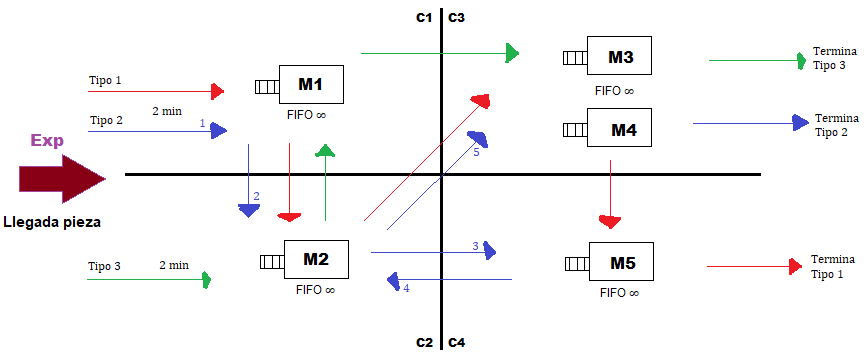
\includegraphics{./imagenes/Esquema_siste_ms.png} Asumimos FIFO para
cada celula de procesamiento. También explicar que los transportes entre
las distintas células deberían ser tomados como si de otro servicio se
tratase y por lo tanto ser nodos en la red. En ellos ninguna pieza
espera a ser transportada, ya que estos nodos tienen infinitos
servidores y por lo tanto, no tienen cola. Debido a esto, para
simplificar el código y nuestro sistema hemos decidido no tratar el
transporte entre nodos como otro nodo.

A continuación se muestra el código de nuestro simulador.

    \begin{Verbatim}[commandchars=\\\{\}]
{\color{incolor}In [{\color{incolor}14}]:} \PY{k+kn}{import} \PY{n+nn}{numpy} \PY{k}{as} \PY{n+nn}{np}
         \PY{k+kn}{import} \PY{n+nn}{random}
         \PY{k+kn}{import} \PY{n+nn}{queue}
         \PY{k+kn}{import} \PY{n+nn}{math}
\end{Verbatim}


    Este es nuestro generador aleatorio de tiempos de llegada de las piezas.
Son generados con una distribución exponencial con los parametros
obtenidos en el contraste realizado anteriormente. Para ello utilizamos
\texttt{numpy.random.exponential}.

    \begin{Verbatim}[commandchars=\\\{\}]
{\color{incolor}In [{\color{incolor}15}]:} \PY{k}{def} \PY{n+nf}{genArrival}\PY{p}{(}\PY{p}{)}\PY{p}{:}
             \PY{k}{return} \PY{n}{np}\PY{o}{.}\PY{n}{random}\PY{o}{.}\PY{n}{exponential}\PY{p}{(}\PY{l+m+mi}{13}\PY{p}{)}
             \PY{c+c1}{\PYZsh{} debug}
             \PY{k}{global} \PY{n}{times}
             \PY{n}{time} \PY{o}{=} \PY{n}{times}\PY{p}{[}\PY{l+m+mi}{0}\PY{p}{]}
             \PY{n}{times} \PY{o}{=} \PY{n}{times}\PY{p}{[}\PY{l+m+mi}{1}\PY{p}{:}\PY{p}{]}
             \PY{k}{return} \PY{n}{time}
\end{Verbatim}


    El tipo de pieza se generará de forma aleatoria, pero siguiendo la
proporción que muestra el archivo \texttt{E1.piezas.txt} que se nos
entrega con el enunciado.

    \begin{Verbatim}[commandchars=\\\{\}]
{\color{incolor}In [{\color{incolor}16}]:} \PY{k}{def} \PY{n+nf}{genPieceType}\PY{p}{(}\PY{p}{)}\PY{p}{:}
             \PY{n}{x} \PY{o}{=} \PY{n}{np}\PY{o}{.}\PY{n}{random}\PY{o}{.}\PY{n}{random}\PY{p}{(}\PY{p}{)}
             \PY{k}{if} \PY{n}{x} \PY{o}{\PYZlt{}} \PY{l+m+mf}{0.2508}\PY{p}{:} \PY{c+c1}{\PYZsh{} 1254/5000}
                 \PY{k}{return} \PY{l+m+mi}{1}
             \PY{k}{elif} \PY{n}{x} \PY{o}{\PYZlt{}} \PY{l+m+mf}{0.7322}\PY{p}{:} \PY{c+c1}{\PYZsh{} (1254+2407)/5000}
                 \PY{k}{return} \PY{l+m+mi}{2}
             \PY{k}{else}\PY{p}{:} \PY{c+c1}{\PYZsh{} x \PYZlt{} 1 (1254+2407+1339)}
                 \PY{k}{return} \PY{l+m+mi}{3}
\end{Verbatim}


    Como nos indica el enunciado los tiempos de procesado de cada pieza en
cada célula siguen una distribución triangular de los tiempos expresados
en minutos de la tabla del enunciado. Para ello utilizamos
\texttt{numpy.random.triangular}.

    \begin{Verbatim}[commandchars=\\\{\}]
{\color{incolor}In [{\color{incolor}17}]:} \PY{k}{class} \PY{n+nc}{System}\PY{p}{(}\PY{p}{)}\PY{p}{:}
             
             \PY{k}{def} \PY{n+nf}{\PYZus{}\PYZus{}init\PYZus{}\PYZus{}}\PY{p}{(}\PY{n+nb+bp}{self}\PY{p}{,} \PY{n}{transportTime}\PY{p}{,} \PY{n}{num\PYZus{}machines}\PY{p}{)}\PY{p}{:}
                 \PY{n+nb+bp}{self}\PY{o}{.}\PY{n}{eventsQueue} \PY{o}{=} \PY{n}{queue}\PY{o}{.}\PY{n}{PriorityQueue}\PY{p}{(}\PY{p}{)}
                 
                 \PY{c+c1}{\PYZsh{} fabrication sequence for each type of piece}
                 \PY{n+nb+bp}{self}\PY{o}{.}\PY{n}{steps} \PY{o}{=} \PY{p}{[}\PY{p}{[}\PY{l+m+mi}{0}\PY{p}{,}\PY{l+m+mi}{1}\PY{p}{,}\PY{l+m+mi}{2}\PY{p}{,}\PY{l+m+mi}{3}\PY{p}{]}\PY{p}{,}
                               \PY{p}{[}\PY{l+m+mi}{0}\PY{p}{,}\PY{l+m+mi}{1}\PY{p}{,}\PY{l+m+mi}{3}\PY{p}{,}\PY{l+m+mi}{1}\PY{p}{,}\PY{l+m+mi}{2}\PY{p}{]}\PY{p}{,}
                               \PY{p}{[}\PY{l+m+mi}{1}\PY{p}{,}\PY{l+m+mi}{0}\PY{p}{,}\PY{l+m+mi}{2}\PY{p}{]}\PY{p}{]}
                 
                 \PY{c+c1}{\PYZsh{} processing times for each type of piece at each step of its phabrication sequence}
                 \PY{n+nb+bp}{self}\PY{o}{.}\PY{n}{processingTimes} \PY{o}{=}\PY{p}{[}\PY{p}{[}\PY{p}{(}\PY{l+m+mi}{6}\PY{p}{,}\PY{l+m+mi}{9}\PY{p}{,}\PY{l+m+mi}{10}\PY{p}{)}\PY{p}{,} \PY{p}{(}\PY{l+m+mi}{5}\PY{p}{,}\PY{l+m+mi}{8}\PY{p}{,}\PY{l+m+mi}{10}\PY{p}{)}\PY{p}{,} \PY{p}{(}\PY{l+m+mi}{15}\PY{p}{,}\PY{l+m+mi}{20}\PY{p}{,}\PY{l+m+mi}{25}\PY{p}{)}\PY{p}{,} \PY{p}{(}\PY{l+m+mi}{8}\PY{p}{,}\PY{l+m+mi}{12}\PY{p}{,}\PY{l+m+mi}{16}\PY{p}{)}\PY{p}{]}\PY{p}{,}
                                    \PY{p}{[}\PY{p}{(}\PY{l+m+mi}{1}\PY{p}{,}\PY{l+m+mi}{13}\PY{p}{,}\PY{l+m+mi}{15}\PY{p}{)}\PY{p}{,} \PY{p}{(}\PY{l+m+mi}{4}\PY{p}{,}\PY{l+m+mi}{6}\PY{p}{,}\PY{l+m+mi}{8}\PY{p}{)}\PY{p}{,} \PY{p}{(}\PY{l+m+mi}{15}\PY{p}{,}\PY{l+m+mi}{18}\PY{p}{,}\PY{l+m+mi}{21}\PY{p}{)}\PY{p}{,} \PY{p}{(}\PY{l+m+mi}{6}\PY{p}{,}\PY{l+m+mi}{9}\PY{p}{,}\PY{l+m+mi}{12}\PY{p}{)}\PY{p}{,} \PY{p}{(}\PY{l+m+mi}{27}\PY{p}{,}\PY{l+m+mi}{30}\PY{p}{,}\PY{l+m+mi}{39}\PY{p}{)}\PY{p}{]}\PY{p}{,} \PY{c+c1}{\PYZsh{} El 30 es un 3 en el enunciado, errata}
                                    \PY{p}{[}\PY{p}{(}\PY{l+m+mi}{7}\PY{p}{,}\PY{l+m+mi}{9}\PY{p}{,}\PY{l+m+mi}{11}\PY{p}{)}\PY{p}{,} \PY{p}{(}\PY{l+m+mi}{7}\PY{p}{,}\PY{l+m+mi}{10}\PY{p}{,}\PY{l+m+mi}{13}\PY{p}{)}\PY{p}{,} \PY{p}{(}\PY{l+m+mi}{18}\PY{p}{,}\PY{l+m+mi}{23}\PY{p}{,}\PY{l+m+mi}{28}\PY{p}{)}\PY{p}{]}\PY{p}{]}
                 
                 
                 \PY{c+c1}{\PYZsh{} cell queues}
                 \PY{n+nb+bp}{self}\PY{o}{.}\PY{n}{queue} \PY{o}{=} \PY{p}{[}\PY{n}{queue}\PY{o}{.}\PY{n}{Queue}\PY{p}{(}\PY{p}{)}\PY{p}{,}\PY{n}{queue}\PY{o}{.}\PY{n}{Queue}\PY{p}{(}\PY{p}{)}\PY{p}{,}\PY{n}{queue}\PY{o}{.}\PY{n}{Queue}\PY{p}{(}\PY{p}{)}\PY{p}{,}\PY{n}{queue}\PY{o}{.}\PY{n}{Queue}\PY{p}{(}\PY{p}{)}\PY{p}{]}
                 
                 \PY{c+c1}{\PYZsh{} number of machines in each cell}
                 \PY{n+nb+bp}{self}\PY{o}{.}\PY{n}{num\PYZus{}machines} \PY{o}{=} \PY{n}{num\PYZus{}machines}
                 
                 \PY{c+c1}{\PYZsh{} number of idle machines in each clell}
                 \PY{n+nb+bp}{self}\PY{o}{.}\PY{n}{idle\PYZus{}machines} \PY{o}{=} \PY{p}{[}\PY{p}{[}\PY{k+kc}{True} \PY{k}{for} \PY{n}{j} \PY{o+ow}{in} \PY{n+nb}{range}\PY{p}{(}\PY{n}{num\PYZus{}machines}\PY{p}{[}\PY{n}{i}\PY{p}{]}\PY{p}{)}\PY{p}{]} \PY{k}{for} \PY{n}{i} \PY{o+ow}{in} \PY{n+nb}{range}\PY{p}{(}\PY{l+m+mi}{4}\PY{p}{)}\PY{p}{]}
                 
                 \PY{c+c1}{\PYZsh{} transportation time between cells}
                 \PY{n+nb+bp}{self}\PY{o}{.}\PY{n}{transportTime} \PY{o}{=} \PY{n}{transportTime}
                 
                 \PY{c+c1}{\PYZsh{} stats counters}
                 \PY{n+nb+bp}{self}\PY{o}{.}\PY{n}{minTime} \PY{o}{=} \PY{p}{[}\PY{n}{math}\PY{o}{.}\PY{n}{inf}\PY{p}{,} \PY{n}{math}\PY{o}{.}\PY{n}{inf}\PY{p}{,} \PY{n}{math}\PY{o}{.}\PY{n}{inf}\PY{p}{]} \PY{c+c1}{\PYZsh{} min processing type of each type of piece}
                 \PY{n+nb+bp}{self}\PY{o}{.}\PY{n}{maxTime} \PY{o}{=} \PY{p}{[}\PY{l+m+mi}{0}\PY{p}{,}\PY{l+m+mi}{0}\PY{p}{,}\PY{l+m+mi}{0}\PY{p}{]} \PY{c+c1}{\PYZsh{} max processing type of each type of piece}
                 \PY{n+nb+bp}{self}\PY{o}{.}\PY{n}{sumTimes} \PY{o}{=} \PY{p}{[}\PY{l+m+mi}{0}\PY{p}{,}\PY{l+m+mi}{0}\PY{p}{,}\PY{l+m+mi}{0}\PY{p}{]} \PY{c+c1}{\PYZsh{} Sum of the processing times of all pieces for each type of piece}
                 \PY{n+nb+bp}{self}\PY{o}{.}\PY{n}{numPieces} \PY{o}{=} \PY{p}{[}\PY{l+m+mi}{0}\PY{p}{,}\PY{l+m+mi}{0}\PY{p}{,}\PY{l+m+mi}{0}\PY{p}{]} \PY{c+c1}{\PYZsh{} Total number of pieces processed for each type of piece}
                 
                 \PY{c+c1}{\PYZsh{} like the area under the integral of the size of each queue over time, but discrete}
                 \PY{n+nb+bp}{self}\PY{o}{.}\PY{n}{queueSizeOverTime} \PY{o}{=} \PY{p}{[}\PY{l+m+mi}{0}\PY{p}{,}\PY{l+m+mi}{0}\PY{p}{,}\PY{l+m+mi}{0}\PY{p}{,}\PY{l+m+mi}{0}\PY{p}{]} 
                 \PY{n+nb+bp}{self}\PY{o}{.}\PY{n}{lastUpdate} \PY{o}{=} \PY{p}{[}\PY{l+m+mi}{0}\PY{p}{,}\PY{l+m+mi}{0}\PY{p}{,}\PY{l+m+mi}{0}\PY{p}{,}\PY{l+m+mi}{0}\PY{p}{]} \PY{c+c1}{\PYZsh{} Last time the previous counter was updated}
                 
                 \PY{n+nb+bp}{self}\PY{o}{.}\PY{n}{idleTime} \PY{o}{=} \PY{p}{[}\PY{p}{[}\PY{l+m+mi}{0} \PY{k}{for} \PY{n}{j} \PY{o+ow}{in} \PY{n+nb}{range}\PY{p}{(}\PY{n}{num\PYZus{}machines}\PY{p}{[}\PY{n}{i}\PY{p}{]}\PY{p}{)}\PY{p}{]} \PY{k}{for} \PY{n}{i} \PY{o+ow}{in} \PY{n+nb}{range}\PY{p}{(}\PY{l+m+mi}{4}\PY{p}{)}\PY{p}{]} \PY{c+c1}{\PYZsh{} total time the}
                                                                     \PY{c+c1}{\PYZsh{} machine j in cell i have been idle}
                 \PY{n+nb+bp}{self}\PY{o}{.}\PY{n}{lastUpdateMachine} \PY{o}{=} \PY{p}{[}\PY{p}{[}\PY{l+m+mi}{0} \PY{k}{for} \PY{n}{j} \PY{o+ow}{in} \PY{n+nb}{range}\PY{p}{(}\PY{n}{num\PYZus{}machines}\PY{p}{[}\PY{n}{i}\PY{p}{]}\PY{p}{)}\PY{p}{]} \PY{k}{for} \PY{n}{i} \PY{o+ow}{in} \PY{n+nb}{range}\PY{p}{(}\PY{l+m+mi}{4}\PY{p}{)}\PY{p}{]} \PY{c+c1}{\PYZsh{} Last time}
                                                                             \PY{c+c1}{\PYZsh{} the previous counter was updated}
                 
                 \PY{n+nb+bp}{self}\PY{o}{.}\PY{n}{debug} \PY{o}{=} \PY{k+kc}{False}
                 
             \PY{c+c1}{\PYZsh{} destructor}
                 \PY{c+c1}{\PYZsh{} close files}
         
             \PY{k}{def} \PY{n+nf}{simul\PYZus{}main}\PY{p}{(}\PY{n+nb+bp}{self}\PY{p}{,}\PY{n}{simulationTime}\PY{p}{)}\PY{p}{:}
             
                 \PY{n+nb+bp}{self}\PY{o}{.}\PY{n}{time} \PY{o}{=} \PY{l+m+mi}{0}
                 
                 \PY{n+nb+bp}{self}\PY{o}{.}\PY{n}{simulationTime} \PY{o}{=} \PY{n}{simulationTime}
                 
                 \PY{n+nb+bp}{self}\PY{o}{.}\PY{n}{nextPiece}\PY{p}{(}\PY{p}{)}
             
                 \PY{k}{while} \PY{o+ow}{not} \PY{n+nb+bp}{self}\PY{o}{.}\PY{n}{eventsQueue}\PY{o}{.}\PY{n}{empty}\PY{p}{(}\PY{p}{)}\PY{p}{:}
                     \PY{n+nb+bp}{self}\PY{o}{.}\PY{n}{time}\PY{p}{,} \PY{n}{\PYZus{}}\PY{p}{,} \PY{n}{nextEvent} \PY{o}{=} \PY{n+nb+bp}{self}\PY{o}{.}\PY{n}{eventsQueue}\PY{o}{.}\PY{n}{get}\PY{p}{(}\PY{p}{)}
                     \PY{n}{nextEvent}\PY{p}{(}\PY{p}{)}
                     
             \PY{k}{def} \PY{n+nf}{simul\PYZus{}main\PYZus{}debug}\PY{p}{(}\PY{n+nb+bp}{self}\PY{p}{,} \PY{n}{simulationTime}\PY{p}{)}\PY{p}{:}
                     
                 \PY{n+nb+bp}{self}\PY{o}{.}\PY{n}{time} \PY{o}{=} \PY{l+m+mi}{0}
             
                 \PY{n+nb+bp}{self}\PY{o}{.}\PY{n}{simulationTime} \PY{o}{=} \PY{n}{simulationTime}
             
                 \PY{n+nb+bp}{self}\PY{o}{.}\PY{n}{nextPiece}\PY{p}{(}\PY{p}{)}
                     
             \PY{k}{def} \PY{n+nf}{debug\PYZus{}step}\PY{p}{(}\PY{n+nb+bp}{self}\PY{p}{)}\PY{p}{:}
                 
                 \PY{k}{if} \PY{o+ow}{not} \PY{n+nb+bp}{self}\PY{o}{.}\PY{n}{eventsQueue}\PY{o}{.}\PY{n}{empty}\PY{p}{(}\PY{p}{)}\PY{p}{:}
                     \PY{n+nb+bp}{self}\PY{o}{.}\PY{n}{time}\PY{p}{,} \PY{n}{eventDescription}\PY{p}{,} \PY{n}{nextEvent} \PY{o}{=} \PY{n+nb+bp}{self}\PY{o}{.}\PY{n}{eventsQueue}\PY{o}{.}\PY{n}{get}\PY{p}{(}\PY{p}{)}
                     \PY{n+nb}{print}\PY{p}{(}\PY{n+nb+bp}{self}\PY{o}{.}\PY{n}{time}\PY{p}{)}
                     \PY{n+nb}{print}\PY{p}{(}\PY{n}{eventDescription}\PY{p}{)}
                     \PY{n}{nextEvent}\PY{p}{(}\PY{p}{)}
                 
             \PY{k}{def} \PY{n+nf}{nextPiece}\PY{p}{(}\PY{n+nb+bp}{self}\PY{p}{)}\PY{p}{:}
                 \PY{n}{nextArrival} \PY{o}{=} \PY{n+nb+bp}{self}\PY{o}{.}\PY{n}{timeTillNextArrival}\PY{p}{(}\PY{p}{)}
                 \PY{n}{nextArrivalTime} \PY{o}{=} \PY{n+nb+bp}{self}\PY{o}{.}\PY{n}{time} \PY{o}{+} \PY{n}{nextArrival}
                 \PY{k}{if} \PY{n}{nextArrivalTime} \PY{o}{\PYZlt{}} \PY{n+nb+bp}{self}\PY{o}{.}\PY{n}{simulationTime}\PY{p}{:}
                     \PY{n}{nextPieceType} \PY{o}{=} \PY{n+nb+bp}{self}\PY{o}{.}\PY{n}{nextPieceType}\PY{p}{(}\PY{p}{)}
                     \PY{n}{nextPiece} \PY{o}{=} \PY{p}{(}\PY{n}{nextArrivalTime}\PY{p}{,} \PY{n}{nextPieceType}\PY{p}{,} \PY{l+m+mi}{0}\PY{p}{)}
                     \PY{c+c1}{\PYZsh{} The prority queue as it is breaks if two events happen at the same time}
                     \PY{n}{eventDescription} \PY{o}{=} \PY{l+s+s2}{\PYZdq{}}\PY{l+s+s2}{piece }\PY{l+s+s2}{\PYZdq{}} \PY{o}{+} \PY{n+nb}{str}\PY{p}{(}\PY{n}{nextPiece}\PY{p}{)} \PY{o}{+} \PY{l+s+s2}{\PYZdq{}}\PY{l+s+s2}{ arrives}\PY{l+s+s2}{\PYZdq{}}
                     \PY{n}{event} \PY{o}{=} \PY{k}{lambda} \PY{p}{:} \PY{n+nb+bp}{self}\PY{o}{.}\PY{n}{arrivePiece}\PY{p}{(}\PY{n}{nextPiece}\PY{p}{)}
                     \PY{n+nb+bp}{self}\PY{o}{.}\PY{n}{eventsQueue}\PY{o}{.}\PY{n}{put}\PY{p}{(}\PY{p}{(}\PY{n}{nextArrivalTime}\PY{p}{,} \PY{n}{eventDescription}\PY{p}{,} \PY{n}{event}\PY{p}{)}\PY{p}{)}
             
             \PY{k}{def} \PY{n+nf}{arrivePiece}\PY{p}{(}\PY{n+nb+bp}{self}\PY{p}{,}\PY{n}{piece}\PY{p}{)}\PY{p}{:}
                 \PY{n+nb+bp}{self}\PY{o}{.}\PY{n}{nextPiece}\PY{p}{(}\PY{p}{)}
                 \PY{n+nb+bp}{self}\PY{o}{.}\PY{n}{advancePiece}\PY{p}{(}\PY{n}{piece}\PY{p}{)}
                 
             \PY{k}{def} \PY{n+nf}{nextPieceType}\PY{p}{(}\PY{n+nb+bp}{self}\PY{p}{)}\PY{p}{:}
                     \PY{k}{return} \PY{n}{genPieceType}\PY{p}{(}\PY{p}{)}\PY{o}{\PYZhy{}}\PY{l+m+mi}{1}
                 \PY{c+c1}{\PYZsh{} Types of pieces are shifted so that the first one is 0}
                 
             \PY{k}{def} \PY{n+nf}{timeTillNextArrival}\PY{p}{(}\PY{n+nb+bp}{self}\PY{p}{)}\PY{p}{:}
                     \PY{k}{return} \PY{n}{genArrival}\PY{p}{(}\PY{p}{)}
             
             \PY{k}{def} \PY{n+nf}{advancePiece}\PY{p}{(}\PY{n+nb+bp}{self}\PY{p}{,}\PY{n}{piece}\PY{p}{)}\PY{p}{:}
                 
                 \PY{n}{arrivalTime}\PY{p}{,} \PY{n}{pieceType}\PY{p}{,} \PY{n}{step} \PY{o}{=} \PY{n}{piece}
         
                 \PY{k}{if} \PY{n+nb+bp}{self}\PY{o}{.}\PY{n}{steps}\PY{p}{[}\PY{n}{pieceType}\PY{p}{]}\PY{p}{[}\PY{n}{step}\PY{p}{:}\PY{p}{]} \PY{o}{==} \PY{p}{[}\PY{p}{]}\PY{p}{:}
                     \PY{n+nb+bp}{self}\PY{o}{.}\PY{n}{finishPiece}\PY{p}{(}\PY{n}{piece}\PY{p}{)}
                     \PY{k}{if} \PY{n+nb+bp}{self}\PY{o}{.}\PY{n}{debug}\PY{p}{:}
                         \PY{n+nb}{print}\PY{p}{(}\PY{l+s+s2}{\PYZdq{}}\PY{l+s+s2}{piece }\PY{l+s+s2}{\PYZdq{}} \PY{o}{+} \PY{n+nb}{str}\PY{p}{(}\PY{n}{arrivalTime}\PY{p}{)} \PY{o}{+} \PY{l+s+s2}{\PYZdq{}}\PY{l+s+s2}{ finishes}\PY{l+s+s2}{\PYZdq{}}\PY{p}{)}
                 \PY{k}{else}\PY{p}{:}
                     \PY{n}{next\PYZus{}cell} \PY{o}{=} \PY{n+nb+bp}{self}\PY{o}{.}\PY{n}{steps}\PY{p}{[}\PY{n}{pieceType}\PY{p}{]}\PY{p}{[}\PY{n}{step}\PY{p}{]}
                     \PY{k}{if} \PY{n}{step} \PY{o}{==} \PY{l+m+mi}{0}\PY{p}{:}
                         \PY{n+nb+bp}{self}\PY{o}{.}\PY{n}{enter}\PY{p}{(}\PY{n}{next\PYZus{}cell}\PY{p}{,}\PY{n}{piece}\PY{p}{)}
                     \PY{k}{else}\PY{p}{:}
                         \PY{n}{eventTime} \PY{o}{=} \PY{n+nb+bp}{self}\PY{o}{.}\PY{n}{time} \PY{o}{+} \PY{n+nb+bp}{self}\PY{o}{.}\PY{n}{transportTime}
                         \PY{n}{eventDescription} \PY{o}{=} \PY{l+s+s2}{\PYZdq{}}\PY{l+s+s2}{piece }\PY{l+s+s2}{\PYZdq{}} \PY{o}{+} \PY{n+nb}{str}\PY{p}{(}\PY{n}{piece}\PY{p}{)} \PY{o}{+} \PY{l+s+s2}{\PYZdq{}}\PY{l+s+s2}{ enters cell }\PY{l+s+s2}{\PYZdq{}} \PY{o}{+} \PY{n+nb}{str}\PY{p}{(}\PY{n}{next\PYZus{}cell}\PY{p}{)}
                         \PY{n}{event} \PY{o}{=} \PY{k}{lambda} \PY{p}{:} \PY{n+nb+bp}{self}\PY{o}{.}\PY{n}{enter}\PY{p}{(}\PY{n}{next\PYZus{}cell}\PY{p}{,}\PY{n}{piece}\PY{p}{)}
                         \PY{n+nb+bp}{self}\PY{o}{.}\PY{n}{eventsQueue}\PY{o}{.}\PY{n}{put}\PY{p}{(}\PY{p}{(}\PY{n}{eventTime}\PY{p}{,} \PY{n}{eventDescription}\PY{p}{,} \PY{n}{event}\PY{p}{)}\PY{p}{)}
             
             \PY{k}{def} \PY{n+nf}{finishPiece}\PY{p}{(}\PY{n+nb+bp}{self}\PY{p}{,}\PY{n}{piece}\PY{p}{)}\PY{p}{:}
                 
                 \PY{n}{arrivalTime}\PY{p}{,} \PY{n}{pieceType}\PY{p}{,} \PY{n}{\PYZus{}} \PY{o}{=} \PY{n}{piece}
                 
                 \PY{n}{totalTime} \PY{o}{=} \PY{n+nb+bp}{self}\PY{o}{.}\PY{n}{time} \PY{o}{\PYZhy{}} \PY{n}{arrivalTime}
                 
                 \PY{k}{if} \PY{n}{totalTime} \PY{o}{\PYZlt{}} \PY{n+nb+bp}{self}\PY{o}{.}\PY{n}{minTime}\PY{p}{[}\PY{n}{pieceType}\PY{p}{]}\PY{p}{:} \PY{c+c1}{\PYZsh{} use dictionaries, since index needs shifting}
                     \PY{n+nb+bp}{self}\PY{o}{.}\PY{n}{minTime}\PY{p}{[}\PY{n}{pieceType}\PY{p}{]} \PY{o}{=} \PY{n}{totalTime}
                
                 \PY{k}{if} \PY{n}{totalTime} \PY{o}{\PYZgt{}} \PY{n+nb+bp}{self}\PY{o}{.}\PY{n}{maxTime}\PY{p}{[}\PY{n}{pieceType}\PY{p}{]}\PY{p}{:}
                     \PY{n+nb+bp}{self}\PY{o}{.}\PY{n}{maxTime}\PY{p}{[}\PY{n}{pieceType}\PY{p}{]} \PY{o}{=} \PY{n}{totalTime}
                 
                 \PY{n+nb+bp}{self}\PY{o}{.}\PY{n}{sumTimes}\PY{p}{[}\PY{n}{pieceType}\PY{p}{]} \PY{o}{+}\PY{o}{=} \PY{n}{totalTime}
                 
                 \PY{n+nb+bp}{self}\PY{o}{.}\PY{n}{numPieces}\PY{p}{[}\PY{n}{pieceType}\PY{p}{]} \PY{o}{+}\PY{o}{=} \PY{l+m+mi}{1}
                 
             
             \PY{k}{def} \PY{n+nf}{enter}\PY{p}{(}\PY{n+nb+bp}{self}\PY{p}{,}\PY{n}{cell}\PY{p}{,}\PY{n}{piece}\PY{p}{)}\PY{p}{:}
                 
                 \PY{k}{for} \PY{n}{machine} \PY{o+ow}{in} \PY{n+nb}{range}\PY{p}{(}\PY{n+nb+bp}{self}\PY{o}{.}\PY{n}{num\PYZus{}machines}\PY{p}{[}\PY{n}{cell}\PY{p}{]}\PY{p}{)}\PY{p}{:}
                     \PY{k}{if} \PY{n+nb+bp}{self}\PY{o}{.}\PY{n}{idle\PYZus{}machines}\PY{p}{[}\PY{n}{cell}\PY{p}{]}\PY{p}{[}\PY{n}{machine}\PY{p}{]}\PY{p}{:}
                         \PY{n+nb+bp}{self}\PY{o}{.}\PY{n}{process}\PY{p}{(}\PY{n}{cell}\PY{p}{,}\PY{n}{piece}\PY{p}{,}\PY{n}{machine}\PY{p}{)}
                         \PY{k}{return}
                     
                 \PY{n+nb+bp}{self}\PY{o}{.}\PY{n}{queueSizeOverTime}\PY{p}{[}\PY{n}{cell}\PY{p}{]} \PY{o}{+}\PY{o}{=} \PY{n+nb+bp}{self}\PY{o}{.}\PY{n}{queue}\PY{p}{[}\PY{n}{cell}\PY{p}{]}\PY{o}{.}\PY{n}{qsize}\PY{p}{(}\PY{p}{)}\PY{o}{*}\PY{p}{(}\PY{n+nb+bp}{self}\PY{o}{.}\PY{n}{time}\PY{o}{\PYZhy{}}\PY{n+nb+bp}{self}\PY{o}{.}\PY{n}{lastUpdate}\PY{p}{[}\PY{n}{cell}\PY{p}{]}\PY{p}{)}
                 \PY{n+nb+bp}{self}\PY{o}{.}\PY{n}{lastUpdate}\PY{p}{[}\PY{n}{cell}\PY{p}{]} \PY{o}{=} \PY{n+nb+bp}{self}\PY{o}{.}\PY{n}{time}
                 \PY{n+nb+bp}{self}\PY{o}{.}\PY{n}{queue}\PY{p}{[}\PY{n}{cell}\PY{p}{]}\PY{o}{.}\PY{n}{put}\PY{p}{(}\PY{n}{piece}\PY{p}{)}
         
             \PY{k}{def} \PY{n+nf}{process}\PY{p}{(}\PY{n+nb+bp}{self}\PY{p}{,}\PY{n}{cell}\PY{p}{,}\PY{n}{piece}\PY{p}{,}\PY{n}{machine}\PY{p}{)}\PY{p}{:}
                 
                 \PY{n+nb+bp}{self}\PY{o}{.}\PY{n}{idleTime}\PY{p}{[}\PY{n}{cell}\PY{p}{]}\PY{p}{[}\PY{n}{machine}\PY{p}{]} \PY{o}{+}\PY{o}{=} \PY{n+nb+bp}{self}\PY{o}{.}\PY{n}{time} \PY{o}{\PYZhy{}} \PY{n+nb+bp}{self}\PY{o}{.}\PY{n}{lastUpdateMachine}\PY{p}{[}\PY{n}{cell}\PY{p}{]}\PY{p}{[}\PY{n}{machine}\PY{p}{]}
                 \PY{n+nb+bp}{self}\PY{o}{.}\PY{n}{lastUpdateMachine}\PY{p}{[}\PY{n}{cell}\PY{p}{]}\PY{p}{[}\PY{n}{machine}\PY{p}{]} \PY{o}{=} \PY{n+nb+bp}{self}\PY{o}{.}\PY{n}{time}
                 
                 \PY{n}{\PYZus{}}\PY{p}{,} \PY{n}{pieceType}\PY{p}{,} \PY{n}{step} \PY{o}{=} \PY{n}{piece}
                 
                 \PY{n}{low}\PY{p}{,} \PY{n}{mode}\PY{p}{,} \PY{n}{upp} \PY{o}{=} \PY{n+nb+bp}{self}\PY{o}{.}\PY{n}{processingTimes}\PY{p}{[}\PY{n}{pieceType}\PY{p}{]}\PY{p}{[}\PY{n}{step}\PY{p}{]}
                 
                 \PY{k}{if} \PY{n+nb+bp}{self}\PY{o}{.}\PY{n}{debug}\PY{p}{:}
                     \PY{n}{processing\PYZus{}time} \PY{o}{=} \PY{n}{mode}
                 \PY{k}{else}\PY{p}{:}
                     \PY{n}{processing\PYZus{}time} \PY{o}{=} \PY{n}{np}\PY{o}{.}\PY{n}{random}\PY{o}{.}\PY{n}{triangular}\PY{p}{(}\PY{n}{low}\PY{p}{,}\PY{n}{mode}\PY{p}{,}\PY{n}{upp}\PY{p}{)}
                 
                 
                 \PY{n+nb+bp}{self}\PY{o}{.}\PY{n}{idle\PYZus{}machines}\PY{p}{[}\PY{n}{cell}\PY{p}{]}\PY{p}{[}\PY{n}{machine}\PY{p}{]} \PY{o}{=} \PY{k+kc}{False}
                 
                 \PY{n}{eventDescription} \PY{o}{=} \PY{l+s+s2}{\PYZdq{}}\PY{l+s+s2}{piece }\PY{l+s+s2}{\PYZdq{}} \PY{o}{+} \PY{n+nb}{str}\PY{p}{(}\PY{n}{piece}\PY{p}{)} \PY{o}{+} \PY{l+s+s2}{\PYZdq{}}\PY{l+s+s2}{ done in cell }\PY{l+s+s2}{\PYZdq{}} \PY{o}{+} \PY{n+nb}{str}\PY{p}{(}\PY{n}{cell}\PY{p}{)}
                 \PY{n+nb+bp}{self}\PY{o}{.}\PY{n}{eventsQueue}\PY{o}{.}\PY{n}{put}\PY{p}{(}\PY{p}{(}\PY{n+nb+bp}{self}\PY{o}{.}\PY{n}{time}\PY{o}{+}\PY{n}{processing\PYZus{}time}\PY{p}{,} \PY{n}{eventDescription}\PY{p}{,} \PY{k}{lambda} \PY{p}{:} \PY{n+nb+bp}{self}\PY{o}{.}\PY{n}{done}\PY{p}{(}\PY{n}{cell}\PY{p}{,}\PY{n}{piece}\PY{p}{,}\PY{n}{machine}\PY{p}{)}\PY{p}{)}\PY{p}{)}
                 
             \PY{k}{def} \PY{n+nf}{done}\PY{p}{(}\PY{n+nb+bp}{self}\PY{p}{,}\PY{n}{cell}\PY{p}{,}\PY{n}{piece}\PY{p}{,}\PY{n}{machine}\PY{p}{)}\PY{p}{:}
                 
                 \PY{n+nb+bp}{self}\PY{o}{.}\PY{n}{lastUpdateMachine}\PY{p}{[}\PY{n}{cell}\PY{p}{]}\PY{p}{[}\PY{n}{machine}\PY{p}{]} \PY{o}{=} \PY{n+nb+bp}{self}\PY{o}{.}\PY{n}{time}
                 
                 \PY{n+nb+bp}{self}\PY{o}{.}\PY{n}{idle\PYZus{}machines}\PY{p}{[}\PY{n}{cell}\PY{p}{]}\PY{p}{[}\PY{n}{machine}\PY{p}{]} \PY{o}{=} \PY{k+kc}{True}
                 
                 \PY{k}{if} \PY{o+ow}{not} \PY{n+nb+bp}{self}\PY{o}{.}\PY{n}{queue}\PY{p}{[}\PY{n}{cell}\PY{p}{]}\PY{o}{.}\PY{n}{empty}\PY{p}{(}\PY{p}{)}\PY{p}{:}
                     
                     \PY{n+nb+bp}{self}\PY{o}{.}\PY{n}{queueSizeOverTime}\PY{p}{[}\PY{n}{cell}\PY{p}{]} \PY{o}{+}\PY{o}{=} \PY{n+nb+bp}{self}\PY{o}{.}\PY{n}{queue}\PY{p}{[}\PY{n}{cell}\PY{p}{]}\PY{o}{.}\PY{n}{qsize}\PY{p}{(}\PY{p}{)}\PY{o}{*}\PY{p}{(}\PY{n+nb+bp}{self}\PY{o}{.}\PY{n}{time}\PY{o}{\PYZhy{}}\PY{n+nb+bp}{self}\PY{o}{.}\PY{n}{lastUpdate}\PY{p}{[}\PY{n}{cell}\PY{p}{]}\PY{p}{)}
                     \PY{n+nb+bp}{self}\PY{o}{.}\PY{n}{lastUpdate}\PY{p}{[}\PY{n}{cell}\PY{p}{]} \PY{o}{=} \PY{n+nb+bp}{self}\PY{o}{.}\PY{n}{time}
                     \PY{n}{nextPiece} \PY{o}{=} \PY{n+nb+bp}{self}\PY{o}{.}\PY{n}{queue}\PY{p}{[}\PY{n}{cell}\PY{p}{]}\PY{o}{.}\PY{n}{get}\PY{p}{(}\PY{p}{)}
                     \PY{n+nb+bp}{self}\PY{o}{.}\PY{n}{process}\PY{p}{(}\PY{n}{cell}\PY{p}{,}\PY{n}{nextPiece}\PY{p}{,}\PY{n}{machine}\PY{p}{)}
                 
                 \PY{n}{arrivalTime}\PY{p}{,} \PY{n}{pieceType}\PY{p}{,} \PY{n}{step} \PY{o}{=} \PY{n}{piece}
                 \PY{n}{piece} \PY{o}{=} \PY{n}{arrivalTime}\PY{p}{,} \PY{n}{pieceType}\PY{p}{,} \PY{n}{step} \PY{o}{+} \PY{l+m+mi}{1}
                 \PY{n+nb+bp}{self}\PY{o}{.}\PY{n}{advancePiece}\PY{p}{(}\PY{n}{piece}\PY{p}{)}
\end{Verbatim}


    Vamos a probar nuestro simulador durante 60 minutos y mostraremos la
traza de la ejecución del simulador, así como los estadísticos
calculados para este tiempo, con el fin de comprobar que el simulador
funciona como se espera. Para iniciar nuestro simulador necesitamos
llamar a \texttt{System} pasandole como parametros el tiempo de
transporte entre células en minutos (en este caso dos minutos) y una
tupla especificando el número de máquinas de procesado en cada célula.
En nuestro caso una máquina para cada célula, salvo la tercera, que
dispone de dos.

    \begin{Verbatim}[commandchars=\\\{\}]
{\color{incolor}In [{\color{incolor}22}]:} \PY{n}{system} \PY{o}{=} \PY{n}{System}\PY{p}{(}\PY{l+m+mi}{2}\PY{p}{,}\PY{p}{[}\PY{l+m+mi}{1}\PY{p}{,}\PY{l+m+mi}{1}\PY{p}{,}\PY{l+m+mi}{2}\PY{p}{,}\PY{l+m+mi}{1}\PY{p}{]}\PY{p}{)}
         \PY{n}{system}\PY{o}{.}\PY{n}{simul\PYZus{}main\PYZus{}debug}\PY{p}{(}\PY{l+m+mi}{60}\PY{p}{)}
         \PY{n}{system}\PY{o}{.}\PY{n}{debug} \PY{o}{=} \PY{k+kc}{True}
         \PY{k}{for} \PY{n}{\PYZus{}} \PY{o+ow}{in} \PY{n+nb}{range}\PY{p}{(}\PY{l+m+mi}{60}\PY{p}{)}\PY{p}{:}
             \PY{n}{system}\PY{o}{.}\PY{n}{debug\PYZus{}step}\PY{p}{(}\PY{p}{)}
\end{Verbatim}


    \begin{Verbatim}[commandchars=\\\{\}]
31.038711548585376
piece (31.038711548585376, 2, 0) arrives
40.038711548585376
piece (31.038711548585376, 2, 0) done in cell 1
42.038711548585376
piece (31.038711548585376, 2, 1) enters cell 0
47.58742260943695
piece (47.58742260943695, 0, 0) arrives
51.09702291102327
piece (51.09702291102327, 1, 0) arrives
52.038711548585376
piece (31.038711548585376, 2, 1) done in cell 0
54.038711548585376
piece (31.038711548585376, 2, 2) enters cell 2
61.038711548585376
piece (47.58742260943695, 0, 0) done in cell 0
63.038711548585376
piece (47.58742260943695, 0, 1) enters cell 1
71.03871154858538
piece (47.58742260943695, 0, 1) done in cell 1
73.03871154858538
piece (47.58742260943695, 0, 2) enters cell 2
74.03871154858538
piece (51.09702291102327, 1, 0) done in cell 0
76.03871154858538
piece (51.09702291102327, 1, 1) enters cell 1
77.03871154858538
piece (31.038711548585376, 2, 2) done in cell 2
piece 31.038711548585376 finishes
82.03871154858538
piece (51.09702291102327, 1, 1) done in cell 1
84.03871154858538
piece (51.09702291102327, 1, 2) enters cell 3
93.03871154858538
piece (47.58742260943695, 0, 2) done in cell 2
95.03871154858538
piece (47.58742260943695, 0, 3) enters cell 3
102.03871154858538
piece (51.09702291102327, 1, 2) done in cell 3
104.03871154858538
piece (51.09702291102327, 1, 3) enters cell 1
113.03871154858538
piece (51.09702291102327, 1, 3) done in cell 1
114.03871154858538
piece (47.58742260943695, 0, 3) done in cell 3
piece 47.58742260943695 finishes
115.03871154858538
piece (51.09702291102327, 1, 4) enters cell 2
145.03871154858538
piece (51.09702291102327, 1, 4) done in cell 2
piece 51.09702291102327 finishes

    \end{Verbatim}

    \begin{Verbatim}[commandchars=\\\{\}]
{\color{incolor}In [{\color{incolor}19}]:} \PY{n+nb}{print}\PY{p}{(}\PY{l+s+s2}{\PYZdq{}}\PY{l+s+s2}{Tiempo (m) de ejecución de la simulación = }\PY{l+s+si}{\PYZpc{}s}\PY{l+s+s2}{\PYZdq{}} \PY{o}{\PYZpc{}}\PY{k}{system}.time\PY{o}{)}
         \PY{n+nb}{print}\PY{p}{(}\PY{l+s+s2}{\PYZdq{}}\PY{l+s+s2}{Tiempo (m) mínimo de fabricación para cada tipo de pieza = }\PY{l+s+si}{\PYZpc{}s}\PY{l+s+s2}{\PYZdq{}} \PY{o}{\PYZpc{}}\PY{k}{system}.minTime\PY{o}{)}
         \PY{n+nb}{print}\PY{p}{(}\PY{l+s+s2}{\PYZdq{}}\PY{l+s+s2}{Tiempo (m) máximo de fabricación para cada tipo de pieza = }\PY{l+s+si}{\PYZpc{}s}\PY{l+s+s2}{\PYZdq{}} \PY{o}{\PYZpc{}}\PY{k}{system}.maxTime\PY{o}{)}
         \PY{n+nb}{print}\PY{p}{(}\PY{l+s+s2}{\PYZdq{}}\PY{l+s+s2}{Suma de los tiempos (m) de procesamiento de todas las piezas de cada tipo = }\PY{l+s+si}{\PYZpc{}s}\PY{l+s+s2}{\PYZdq{}} \PY{o}{\PYZpc{}}\PY{k}{system}.sumTimes\PY{o}{)}
         \PY{n+nb}{print}\PY{p}{(}\PY{l+s+s2}{\PYZdq{}}\PY{l+s+s2}{Cantidad de piezas fabricadas de cada tipo = }\PY{l+s+si}{\PYZpc{}s}\PY{l+s+s2}{\PYZdq{}} \PY{o}{\PYZpc{}}\PY{k}{system}.numPieces\PY{o}{)}
         \PY{n+nb}{print}\PY{p}{(}\PY{l+s+s2}{\PYZdq{}}\PY{l+s+s2}{Tiempo (m) medio de fabricación para cada tipo de pieza = }\PY{l+s+si}{\PYZpc{}s}\PY{l+s+s2}{\PYZdq{}} \PY{o}{\PYZpc{}}\PY{p}{[}\PY{n}{system}\PY{o}{.}\PY{n}{sumTimes}\PY{p}{[}\PY{n}{i}\PY{p}{]}\PY{o}{/}\PY{n}{system}\PY{o}{.}\PY{n}{numPieces}\PY{p}{[}\PY{n}{i}\PY{p}{]} \PY{k}{for} \PY{n}{i} \PY{o+ow}{in} \PY{n+nb}{range}\PY{p}{(}\PY{l+m+mi}{3}\PY{p}{)}\PY{p}{]}\PY{p}{)}
         \PY{n+nb}{print}\PY{p}{(}\PY{l+s+s2}{\PYZdq{}}\PY{l+s+s2}{Número medio de piezas esperando en cada célula = }\PY{l+s+si}{\PYZpc{}s}\PY{l+s+s2}{\PYZdq{}} \PY{o}{\PYZpc{}}\PY{p}{[}\PY{n}{system}\PY{o}{.}\PY{n}{queueSizeOverTime}\PY{p}{[}\PY{n}{i}\PY{p}{]}\PY{o}{/}\PY{n}{system}\PY{o}{.}\PY{n}{time} \PY{k}{for} \PY{n}{i} \PY{o+ow}{in} \PY{n+nb}{range}\PY{p}{(}\PY{l+m+mi}{4}\PY{p}{)}\PY{p}{]}\PY{p}{)}
         \PY{n+nb}{print}\PY{p}{(}\PY{l+s+s2}{\PYZdq{}}\PY{l+s+s2}{Tiempo (m) que están ociosas cada máquina de cada células = }\PY{l+s+si}{\PYZpc{}s}\PY{l+s+s2}{\PYZdq{}} \PY{o}{\PYZpc{}}\PY{k}{system}.idleTime\PY{o}{)}
\end{Verbatim}


    \begin{Verbatim}[commandchars=\\\{\}]
Tiempo (m) de ejecución de la simulación = 139.1146418207905
Tiempo (m) mínimo de fabricación para cada tipo de pieza = [55.0, 92.96279481200423, 54.382476098065936]
Tiempo (m) máximo de fabricación para cada tipo de pieza = [55.0, 101.78321070674541, 54.382476098065936]
Suma de los tiempos (m) de procesamiento de todas las piezas de cada tipo = [55.0, 194.74600551874966, 54.382476098065936]
Cantidad de piezas fabricadas de cada tipo = [1, 2, 1]
Tiempo (m) medio de fabricación para cada tipo de pieza = [55.0, 97.37300275937483, 54.382476098065936]
Número medio de piezas esperando en cada célula = [0.09463911657675536, 0.05174036694961793, 0.02431430691834215, 0.08182083459431257]
Tiempo (m) que están ociosas cada máquina de cada células = [[10.11464182079051], [60.11464182079051], [86.11464182079051, 44.11464182079051], [48.11464182079051]]

    \end{Verbatim}

    Observando la traza y las estadísticas comprobamos que funciona como se
espera.

    \subsubsection{Apartado A: Tiempo de transporte = 2
min.}\label{apartado-a-tiempo-de-transporte-2-min.}

    En este apartado simulamos el comportamiento del sistema durante 2
meses, suponiendo que el taller trabaja de forma ininterrumpida, y
calculamos el tiempo mínimo, medio y máximo que tardan en fabricarse los
tres tipos de piezas, el número medio de piezas esperando en cada una de
las 4 células y la proporción de tiempo que están ociosas las máquinas
de procesado de las células.

    \begin{Verbatim}[commandchars=\\\{\}]
{\color{incolor}In [{\color{incolor}27}]:} \PY{n}{system} \PY{o}{=} \PY{n}{System}\PY{p}{(}\PY{l+m+mi}{2}\PY{p}{,}\PY{p}{[}\PY{l+m+mi}{1}\PY{p}{,}\PY{l+m+mi}{1}\PY{p}{,}\PY{l+m+mi}{2}\PY{p}{,}\PY{l+m+mi}{1}\PY{p}{]}\PY{p}{)}
         \PY{n}{system}\PY{o}{.}\PY{n}{simul\PYZus{}main}\PY{p}{(}\PY{l+m+mi}{86400}\PY{p}{)} \PY{c+c1}{\PYZsh{} 2 months}
\end{Verbatim}


    \begin{Verbatim}[commandchars=\\\{\}]
{\color{incolor}In [{\color{incolor}28}]:} \PY{n+nb}{print}\PY{p}{(}\PY{l+s+s2}{\PYZdq{}}\PY{l+s+s2}{Tiempo (m) de ejecución de la simulación = }\PY{l+s+si}{\PYZpc{}s}\PY{l+s+s2}{\PYZdq{}} \PY{o}{\PYZpc{}}\PY{k}{system}.time\PY{o}{)}
         \PY{n+nb}{print}\PY{p}{(}\PY{l+s+s2}{\PYZdq{}}\PY{l+s+s2}{Tiempo (m) mínimo de fabricación para cada tipo de pieza = }\PY{l+s+si}{\PYZpc{}s}\PY{l+s+s2}{\PYZdq{}} \PY{o}{\PYZpc{}}\PY{k}{system}.minTime\PY{o}{)}
         \PY{n+nb}{print}\PY{p}{(}\PY{l+s+s2}{\PYZdq{}}\PY{l+s+s2}{Tiempo (m) máximo de fabricación para cada tipo de pieza = }\PY{l+s+si}{\PYZpc{}s}\PY{l+s+s2}{\PYZdq{}} \PY{o}{\PYZpc{}}\PY{k}{system}.maxTime\PY{o}{)}
         \PY{n+nb}{print}\PY{p}{(}\PY{l+s+s2}{\PYZdq{}}\PY{l+s+s2}{Suma de los tiempos (m) de procesamiento de todas las piezas de cada tipo = }\PY{l+s+si}{\PYZpc{}s}\PY{l+s+s2}{\PYZdq{}} \PY{o}{\PYZpc{}}\PY{k}{system}.sumTimes\PY{o}{)}
         \PY{n+nb}{print}\PY{p}{(}\PY{l+s+s2}{\PYZdq{}}\PY{l+s+s2}{Cantidad de piezas fabricadas de cada tipo = }\PY{l+s+si}{\PYZpc{}s}\PY{l+s+s2}{\PYZdq{}} \PY{o}{\PYZpc{}}\PY{k}{system}.numPieces\PY{o}{)}
         \PY{n+nb}{print}\PY{p}{(}\PY{l+s+s2}{\PYZdq{}}\PY{l+s+s2}{Tiempo (m) medio de fabricación para cada tipo de pieza = }\PY{l+s+si}{\PYZpc{}s}\PY{l+s+s2}{\PYZdq{}} \PY{o}{\PYZpc{}}\PY{p}{[}\PY{n}{system}\PY{o}{.}\PY{n}{sumTimes}\PY{p}{[}\PY{n}{i}\PY{p}{]}\PY{o}{/}\PY{n}{system}\PY{o}{.}\PY{n}{numPieces}\PY{p}{[}\PY{n}{i}\PY{p}{]} \PY{k}{for} \PY{n}{i} \PY{o+ow}{in} \PY{n+nb}{range}\PY{p}{(}\PY{l+m+mi}{3}\PY{p}{)}\PY{p}{]}\PY{p}{)}
         \PY{n+nb}{print}\PY{p}{(}\PY{l+s+s2}{\PYZdq{}}\PY{l+s+s2}{Número medio de piezas esperando en cada célula = }\PY{l+s+si}{\PYZpc{}s}\PY{l+s+s2}{\PYZdq{}} \PY{o}{\PYZpc{}}\PY{p}{[}\PY{n}{system}\PY{o}{.}\PY{n}{queueSizeOverTime}\PY{p}{[}\PY{n}{i}\PY{p}{]}\PY{o}{/}\PY{n}{system}\PY{o}{.}\PY{n}{time} \PY{k}{for} \PY{n}{i} \PY{o+ow}{in} \PY{n+nb}{range}\PY{p}{(}\PY{l+m+mi}{4}\PY{p}{)}\PY{p}{]}\PY{p}{)}
         \PY{n+nb}{print}\PY{p}{(}\PY{l+s+s2}{\PYZdq{}}\PY{l+s+s2}{Tiempo (m) que están ociosas cada máquina de cada células = }\PY{l+s+si}{\PYZpc{}s}\PY{l+s+s2}{\PYZdq{}} \PY{o}{\PYZpc{}}\PY{k}{system}.idleTime\PY{o}{)}
\end{Verbatim}


    \begin{Verbatim}[commandchars=\\\{\}]
Tiempo (m) de ejecución de la simulación = 89538.41318113472
Tiempo (m) mínimo de fabricación para cada tipo de pieza = [54.01354626103762, 83.92547496801558, 50.14091139228685]
Tiempo (m) máximo de fabricación para cada tipo de pieza = [3486.8641209033667, 3622.116737350734, 3439.5579504233174]
Suma de los tiempos (m) de procesamiento de todas las piezas de cada tipo = [3383844.047498112, 7065541.959060886, 3554196.4137298786]
Cantidad de piezas fabricadas de cada tipo = [1627, 3291, 1787]
Tiempo (m) medio de fabricación para cada tipo de pieza = [2079.8058066982867, 2146.928580693068, 1988.9179707497922]
Número medio de piezas esperando en cada célula = [0.9373724188914588, 3.33888777688316, 144.0467800321743, 3.1375591013934945]
Tiempo (m) que están ociosas cada máquina de cada células = [[23082.400293518207], [8567.766393507693], [71.83326045987015, 79.78724791026757], [10752.841586832921]]

    \end{Verbatim}

    \subsubsection{Apartado B: Tiempo de transporte = 1
min.}\label{apartado-b-tiempo-de-transporte-1-min.}

    En este punto reducimos el tiempo de transporte de 2 minutos a 1 minuto
y calculamos de nuevo las métricas tiempo mínimo, medio y máximo que
tardan en fabricarse los tres tipos de piezas, el número medio de piezas
esperando en cada una de las 4 células y la proporción de tiempo que
están ociosas las máquinas de procesado de las células.

    \begin{Verbatim}[commandchars=\\\{\}]
{\color{incolor}In [{\color{incolor}26}]:} \PY{n}{system} \PY{o}{=} \PY{n}{System}\PY{p}{(}\PY{l+m+mi}{1}\PY{p}{,}\PY{p}{[}\PY{l+m+mi}{1}\PY{p}{,}\PY{l+m+mi}{1}\PY{p}{,}\PY{l+m+mi}{2}\PY{p}{,}\PY{l+m+mi}{1}\PY{p}{]}\PY{p}{)}
         \PY{n}{system}\PY{o}{.}\PY{n}{simul\PYZus{}main}\PY{p}{(}\PY{l+m+mi}{86400}\PY{p}{)} \PY{c+c1}{\PYZsh{} 2 months}
         \PY{n+nb}{print}\PY{p}{(}\PY{l+s+s2}{\PYZdq{}}\PY{l+s+s2}{Tiempo (m) de ejecución de la simulación = }\PY{l+s+si}{\PYZpc{}s}\PY{l+s+s2}{\PYZdq{}} \PY{o}{\PYZpc{}}\PY{k}{system}.time\PY{o}{)}
         \PY{n+nb}{print}\PY{p}{(}\PY{l+s+s2}{\PYZdq{}}\PY{l+s+s2}{Tiempo (m) mínimo de fabricación para cada tipo de pieza = }\PY{l+s+si}{\PYZpc{}s}\PY{l+s+s2}{\PYZdq{}} \PY{o}{\PYZpc{}}\PY{k}{system}.minTime\PY{o}{)}
         \PY{n+nb}{print}\PY{p}{(}\PY{l+s+s2}{\PYZdq{}}\PY{l+s+s2}{Tiempo (m) máximo de fabricación para cada tipo de pieza = }\PY{l+s+si}{\PYZpc{}s}\PY{l+s+s2}{\PYZdq{}} \PY{o}{\PYZpc{}}\PY{k}{system}.maxTime\PY{o}{)}
         \PY{n+nb}{print}\PY{p}{(}\PY{l+s+s2}{\PYZdq{}}\PY{l+s+s2}{Suma de los tiempos (m) de procesamiento de todas las piezas de cada tipo = }\PY{l+s+si}{\PYZpc{}s}\PY{l+s+s2}{\PYZdq{}} \PY{o}{\PYZpc{}}\PY{k}{system}.sumTimes\PY{o}{)}
         \PY{n+nb}{print}\PY{p}{(}\PY{l+s+s2}{\PYZdq{}}\PY{l+s+s2}{Cantidad de piezas fabricadas de cada tipo = }\PY{l+s+si}{\PYZpc{}s}\PY{l+s+s2}{\PYZdq{}} \PY{o}{\PYZpc{}}\PY{k}{system}.numPieces\PY{o}{)}
         \PY{n+nb}{print}\PY{p}{(}\PY{l+s+s2}{\PYZdq{}}\PY{l+s+s2}{Tiempo (m) medio de fabricación para cada tipo de pieza = }\PY{l+s+si}{\PYZpc{}s}\PY{l+s+s2}{\PYZdq{}} \PY{o}{\PYZpc{}}\PY{p}{[}\PY{n}{system}\PY{o}{.}\PY{n}{sumTimes}\PY{p}{[}\PY{n}{i}\PY{p}{]}\PY{o}{/}\PY{n}{system}\PY{o}{.}\PY{n}{numPieces}\PY{p}{[}\PY{n}{i}\PY{p}{]} \PY{k}{for} \PY{n}{i} \PY{o+ow}{in} \PY{n+nb}{range}\PY{p}{(}\PY{l+m+mi}{3}\PY{p}{)}\PY{p}{]}\PY{p}{)}
         \PY{n+nb}{print}\PY{p}{(}\PY{l+s+s2}{\PYZdq{}}\PY{l+s+s2}{Número medio de piezas esperando en cada célula = }\PY{l+s+si}{\PYZpc{}s}\PY{l+s+s2}{\PYZdq{}} \PY{o}{\PYZpc{}}\PY{p}{[}\PY{n}{system}\PY{o}{.}\PY{n}{queueSizeOverTime}\PY{p}{[}\PY{n}{i}\PY{p}{]}\PY{o}{/}\PY{n}{system}\PY{o}{.}\PY{n}{time} \PY{k}{for} \PY{n}{i} \PY{o+ow}{in} \PY{n+nb}{range}\PY{p}{(}\PY{l+m+mi}{4}\PY{p}{)}\PY{p}{]}\PY{p}{)}
         \PY{n+nb}{print}\PY{p}{(}\PY{l+s+s2}{\PYZdq{}}\PY{l+s+s2}{Tiempo (m) que están ociosas cada máquina de cada células = }\PY{l+s+si}{\PYZpc{}s}\PY{l+s+s2}{\PYZdq{}} \PY{o}{\PYZpc{}}\PY{k}{system}.idleTime\PY{o}{)}
\end{Verbatim}


    \begin{Verbatim}[commandchars=\\\{\}]
Tiempo (m) de ejecución de la simulación = 88921.76470960857
Tiempo (m) mínimo de fabricación para cada tipo de pieza = [90.26698482035553, 86.30092987227198, 50.41239912393283]
Tiempo (m) máximo de fabricación para cada tipo de pieza = [2523.888564586392, 2620.3701679258083, 2535.0394305682566]
Suma de los tiempos (m) de procesamiento de todas las piezas de cada tipo = [2162439.835220402, 4298571.708123818, 2174320.434358015]
Cantidad de piezas fabricadas de cada tipo = [1678, 3208, 1796]
Tiempo (m) medio de fabricación para cada tipo de pieza = [1288.7007361265805, 1339.953774352811, 1210.6461215801867]
Número medio de piezas esperando en cada célula = [0.9121623589927585, 2.9223601682732214, 86.0160482315344, 2.572581836389285]
Tiempo (m) que están ociosas cada máquina de cada células = [[23687.272426008887], [9430.585089754606], [92.85054610724163, 89.07338503203395], [10865.390325142325]]

    \end{Verbatim}

    \subsection{Máquina de procesado
adicional}\label{muxe1quina-de-procesado-adicional}

    En caso de que fuese posible disponer de una máquina de procesado
adicional,¿en qué célula sería más beneficioso ponerla?

    A continuación vamos a calcular las mismas métricas que en los apartados
A y B para simulaciones en las que vamos a incluir una o varias máquinas
adicionales en las diferentes células. Mediante la comparativa de los
resultados obtenidos vamos a definir la solución más ventajosa.

    \subsubsection{Caso1\_}\label{caso1_}

    Incluímos una segunda máquina en la célula 1, dejando por tanto 2
máquinas en las células 1 y 3.

    \begin{Verbatim}[commandchars=\\\{\}]
{\color{incolor}In [{\color{incolor}45}]:} \PY{n}{np}\PY{o}{.}\PY{n}{random}\PY{o}{.}\PY{n}{seed}\PY{p}{(}\PY{l+m+mi}{0}\PY{p}{)}
\end{Verbatim}


    \begin{Verbatim}[commandchars=\\\{\}]
{\color{incolor}In [{\color{incolor}46}]:} \PY{n}{system} \PY{o}{=} \PY{n}{System}\PY{p}{(}\PY{l+m+mi}{2}\PY{p}{,}\PY{p}{[}\PY{l+m+mi}{2}\PY{p}{,}\PY{l+m+mi}{1}\PY{p}{,}\PY{l+m+mi}{2}\PY{p}{,}\PY{l+m+mi}{1}\PY{p}{]}\PY{p}{)}
         \PY{n}{system}\PY{o}{.}\PY{n}{simul\PYZus{}main}\PY{p}{(}\PY{l+m+mi}{86400}\PY{p}{)}
\end{Verbatim}


    \begin{Verbatim}[commandchars=\\\{\}]
{\color{incolor}In [{\color{incolor}47}]:} \PY{n+nb}{print}\PY{p}{(}\PY{l+s+s2}{\PYZdq{}}\PY{l+s+s2}{Tiempo (m) de ejecución de la simulación = }\PY{l+s+si}{\PYZpc{}s}\PY{l+s+s2}{\PYZdq{}} \PY{o}{\PYZpc{}}\PY{k}{system}.time\PY{o}{)}
         \PY{n+nb}{print}\PY{p}{(}\PY{l+s+s2}{\PYZdq{}}\PY{l+s+s2}{Tiempo (m) mínimo de fabricación para cada tipo de pieza = }\PY{l+s+si}{\PYZpc{}s}\PY{l+s+s2}{\PYZdq{}} \PY{o}{\PYZpc{}}\PY{k}{system}.minTime\PY{o}{)}
         \PY{n+nb}{print}\PY{p}{(}\PY{l+s+s2}{\PYZdq{}}\PY{l+s+s2}{Tiempo (m) máximo de fabricación para cada tipo de pieza = }\PY{l+s+si}{\PYZpc{}s}\PY{l+s+s2}{\PYZdq{}} \PY{o}{\PYZpc{}}\PY{k}{system}.maxTime\PY{o}{)}
         \PY{n+nb}{print}\PY{p}{(}\PY{l+s+s2}{\PYZdq{}}\PY{l+s+s2}{Suma de los tiempos (m) de procesamiento de todas las piezas de cada tipo = }\PY{l+s+si}{\PYZpc{}s}\PY{l+s+s2}{\PYZdq{}} \PY{o}{\PYZpc{}}\PY{k}{system}.sumTimes\PY{o}{)}
         \PY{n+nb}{print}\PY{p}{(}\PY{l+s+s2}{\PYZdq{}}\PY{l+s+s2}{Cantidad de piezas fabricadas de cada tipo = }\PY{l+s+si}{\PYZpc{}s}\PY{l+s+s2}{\PYZdq{}} \PY{o}{\PYZpc{}}\PY{k}{system}.numPieces\PY{o}{)}
         \PY{n+nb}{print}\PY{p}{(}\PY{l+s+s2}{\PYZdq{}}\PY{l+s+s2}{Tiempo (m) medio de fabricación para cada tipo de pieza = }\PY{l+s+si}{\PYZpc{}s}\PY{l+s+s2}{\PYZdq{}} \PY{o}{\PYZpc{}}\PY{p}{[}\PY{n}{system}\PY{o}{.}\PY{n}{sumTimes}\PY{p}{[}\PY{n}{i}\PY{p}{]}\PY{o}{/}\PY{n}{system}\PY{o}{.}\PY{n}{numPieces}\PY{p}{[}\PY{n}{i}\PY{p}{]} \PY{k}{for} \PY{n}{i} \PY{o+ow}{in} \PY{n+nb}{range}\PY{p}{(}\PY{l+m+mi}{3}\PY{p}{)}\PY{p}{]}\PY{p}{)}
         \PY{n+nb}{print}\PY{p}{(}\PY{l+s+s2}{\PYZdq{}}\PY{l+s+s2}{Número medio de piezas esperando en cada célula = }\PY{l+s+si}{\PYZpc{}s}\PY{l+s+s2}{\PYZdq{}} \PY{o}{\PYZpc{}}\PY{p}{[}\PY{n}{system}\PY{o}{.}\PY{n}{queueSizeOverTime}\PY{p}{[}\PY{n}{i}\PY{p}{]}\PY{o}{/}\PY{n}{system}\PY{o}{.}\PY{n}{time} \PY{k}{for} \PY{n}{i} \PY{o+ow}{in} \PY{n+nb}{range}\PY{p}{(}\PY{l+m+mi}{4}\PY{p}{)}\PY{p}{]}\PY{p}{)}
         \PY{n+nb}{print}\PY{p}{(}\PY{l+s+s2}{\PYZdq{}}\PY{l+s+s2}{Tiempo (m) que están ociosas cada máquina de cada células = }\PY{l+s+si}{\PYZpc{}s}\PY{l+s+s2}{\PYZdq{}} \PY{o}{\PYZpc{}}\PY{k}{system}.idleTime\PY{o}{)}
\end{Verbatim}


    \begin{Verbatim}[commandchars=\\\{\}]
Tiempo (m) de ejecución de la simulación = 89382.39784571007
Tiempo (m) mínimo de fabricación para cada tipo de pieza = [58.74149040832809, 86.46817377192502, 43.430558288539714]
Tiempo (m) máximo de fabricación para cada tipo de pieza = [3523.910004629157, 3577.512329174191, 3443.641387891672]
Suma de los tiempos (m) de procesamiento de todas las piezas de cada tipo = [3631407.7469661664, 7223311.171336805, 3664983.8220654908]
Cantidad de piezas fabricadas de cada tipo = [1683, 3256, 1776]
Tiempo (m) medio de fabricación para cada tipo de pieza = [2157.699196058328, 2218.4616619584785, 2063.6170169287675]
Número medio de piezas esperando en cada célula = [0.05672054710289344, 3.01643365303673, 151.18449845767756, 3.2479941505374215]
Tiempo (m) que están ociosas cada máquina de cada células = [[45437.95781157008, 64095.47445991962], [8803.622896305074], [112.34815473015725, 116.42574050481903], [10471.822431724398]]

    \end{Verbatim}

    \subsubsection{Caso2\_}\label{caso2_}

    Incluímos una segunda máquina en la célula 2, dejando por tanto 2
máquinas en las células 2 y 3.

    \begin{Verbatim}[commandchars=\\\{\}]
{\color{incolor}In [{\color{incolor}48}]:} \PY{n}{np}\PY{o}{.}\PY{n}{random}\PY{o}{.}\PY{n}{seed}\PY{p}{(}\PY{l+m+mi}{0}\PY{p}{)}
\end{Verbatim}


    \begin{Verbatim}[commandchars=\\\{\}]
{\color{incolor}In [{\color{incolor}49}]:} \PY{n}{system} \PY{o}{=} \PY{n}{System}\PY{p}{(}\PY{l+m+mi}{2}\PY{p}{,}\PY{p}{[}\PY{l+m+mi}{1}\PY{p}{,}\PY{l+m+mi}{2}\PY{p}{,}\PY{l+m+mi}{2}\PY{p}{,}\PY{l+m+mi}{1}\PY{p}{]}\PY{p}{)}
         \PY{n}{system}\PY{o}{.}\PY{n}{simul\PYZus{}main}\PY{p}{(}\PY{l+m+mi}{86400}\PY{p}{)}
\end{Verbatim}


    \begin{Verbatim}[commandchars=\\\{\}]
{\color{incolor}In [{\color{incolor}50}]:} \PY{n+nb}{print}\PY{p}{(}\PY{l+s+s2}{\PYZdq{}}\PY{l+s+s2}{Tiempo (m) de ejecución de la simulación = }\PY{l+s+si}{\PYZpc{}s}\PY{l+s+s2}{\PYZdq{}} \PY{o}{\PYZpc{}}\PY{k}{system}.time\PY{o}{)}
         \PY{n+nb}{print}\PY{p}{(}\PY{l+s+s2}{\PYZdq{}}\PY{l+s+s2}{Tiempo (m) mínimo de fabricación para cada tipo de pieza = }\PY{l+s+si}{\PYZpc{}s}\PY{l+s+s2}{\PYZdq{}} \PY{o}{\PYZpc{}}\PY{k}{system}.minTime\PY{o}{)}
         \PY{n+nb}{print}\PY{p}{(}\PY{l+s+s2}{\PYZdq{}}\PY{l+s+s2}{Tiempo (m) máximo de fabricación para cada tipo de pieza = }\PY{l+s+si}{\PYZpc{}s}\PY{l+s+s2}{\PYZdq{}} \PY{o}{\PYZpc{}}\PY{k}{system}.maxTime\PY{o}{)}
         \PY{n+nb}{print}\PY{p}{(}\PY{l+s+s2}{\PYZdq{}}\PY{l+s+s2}{Suma de los tiempos (m) de procesamiento de todas las piezas de cada tipo = }\PY{l+s+si}{\PYZpc{}s}\PY{l+s+s2}{\PYZdq{}} \PY{o}{\PYZpc{}}\PY{k}{system}.sumTimes\PY{o}{)}
         \PY{n+nb}{print}\PY{p}{(}\PY{l+s+s2}{\PYZdq{}}\PY{l+s+s2}{Cantidad de piezas fabricadas de cada tipo = }\PY{l+s+si}{\PYZpc{}s}\PY{l+s+s2}{\PYZdq{}} \PY{o}{\PYZpc{}}\PY{k}{system}.numPieces\PY{o}{)}
         \PY{n+nb}{print}\PY{p}{(}\PY{l+s+s2}{\PYZdq{}}\PY{l+s+s2}{Tiempo (m) medio de fabricación para cada tipo de pieza = }\PY{l+s+si}{\PYZpc{}s}\PY{l+s+s2}{\PYZdq{}} \PY{o}{\PYZpc{}}\PY{p}{[}\PY{n}{system}\PY{o}{.}\PY{n}{sumTimes}\PY{p}{[}\PY{n}{i}\PY{p}{]}\PY{o}{/}\PY{n}{system}\PY{o}{.}\PY{n}{numPieces}\PY{p}{[}\PY{n}{i}\PY{p}{]} \PY{k}{for} \PY{n}{i} \PY{o+ow}{in} \PY{n+nb}{range}\PY{p}{(}\PY{l+m+mi}{3}\PY{p}{)}\PY{p}{]}\PY{p}{)}
         \PY{n+nb}{print}\PY{p}{(}\PY{l+s+s2}{\PYZdq{}}\PY{l+s+s2}{Número medio de piezas esperando en cada célula = }\PY{l+s+si}{\PYZpc{}s}\PY{l+s+s2}{\PYZdq{}} \PY{o}{\PYZpc{}}\PY{p}{[}\PY{n}{system}\PY{o}{.}\PY{n}{queueSizeOverTime}\PY{p}{[}\PY{n}{i}\PY{p}{]}\PY{o}{/}\PY{n}{system}\PY{o}{.}\PY{n}{time} \PY{k}{for} \PY{n}{i} \PY{o+ow}{in} \PY{n+nb}{range}\PY{p}{(}\PY{l+m+mi}{4}\PY{p}{)}\PY{p}{]}\PY{p}{)}
         \PY{n+nb}{print}\PY{p}{(}\PY{l+s+s2}{\PYZdq{}}\PY{l+s+s2}{Tiempo (m) que están ociosas cada máquina de cada células = }\PY{l+s+si}{\PYZpc{}s}\PY{l+s+s2}{\PYZdq{}} \PY{o}{\PYZpc{}}\PY{k}{system}.idleTime\PY{o}{)}
\end{Verbatim}


    \begin{Verbatim}[commandchars=\\\{\}]
Tiempo (m) de ejecución de la simulación = 87887.80376318807
Tiempo (m) mínimo de fabricación para cada tipo de pieza = [51.55413598831865, 82.7936181009909, 41.07770502365565]
Tiempo (m) máximo de fabricación para cada tipo de pieza = [2299.8255717818247, 2285.612935242483, 2173.7939938420823]
Suma de los tiempos (m) de procesamiento de todas las piezas de cada tipo = [2538448.675921374, 4725511.289442616, 2530010.466936053]
Cantidad de piezas fabricadas de cada tipo = [1711, 3117, 1775]
Tiempo (m) medio de fabricación para cada tipo de pieza = [1483.605304454339, 1516.0446870204091, 1425.3580095414382]
Número medio de piezas esperando en cada célula = [0.9339098784999093, 0.039363230360598404, 103.12735602206237, 2.4281905939954496]
Tiempo (m) que están ociosas cada máquina de cada células = [[24651.286137970797], [38455.30815377923, 58643.588027146674], [305.4425364271946, 427.5343531082833], [11243.05995436342]]

    \end{Verbatim}

    \subsubsection{Caso3\_}\label{caso3_}

    Incluímos una tercera máquina en la célula 3, dejando el resto con 1
sóla máquina como originalmente.

    \begin{Verbatim}[commandchars=\\\{\}]
{\color{incolor}In [{\color{incolor}60}]:} \PY{n}{np}\PY{o}{.}\PY{n}{random}\PY{o}{.}\PY{n}{seed}\PY{p}{(}\PY{l+m+mi}{0}\PY{p}{)}
\end{Verbatim}


    \begin{Verbatim}[commandchars=\\\{\}]
{\color{incolor}In [{\color{incolor}61}]:} \PY{n}{system} \PY{o}{=} \PY{n}{System}\PY{p}{(}\PY{l+m+mi}{2}\PY{p}{,}\PY{p}{[}\PY{l+m+mi}{1}\PY{p}{,}\PY{l+m+mi}{1}\PY{p}{,}\PY{l+m+mi}{3}\PY{p}{,}\PY{l+m+mi}{1}\PY{p}{]}\PY{p}{)}
         \PY{n}{system}\PY{o}{.}\PY{n}{simul\PYZus{}main}\PY{p}{(}\PY{l+m+mi}{86400}\PY{p}{)}
\end{Verbatim}


    \begin{Verbatim}[commandchars=\\\{\}]
{\color{incolor}In [{\color{incolor}62}]:} \PY{n+nb}{print}\PY{p}{(}\PY{l+s+s2}{\PYZdq{}}\PY{l+s+s2}{Tiempo (m) de ejecución de la simulación = }\PY{l+s+si}{\PYZpc{}s}\PY{l+s+s2}{\PYZdq{}} \PY{o}{\PYZpc{}}\PY{k}{system}.time\PY{o}{)}
         \PY{n+nb}{print}\PY{p}{(}\PY{l+s+s2}{\PYZdq{}}\PY{l+s+s2}{Tiempo (m) mínimo de fabricación para cada tipo de pieza = }\PY{l+s+si}{\PYZpc{}s}\PY{l+s+s2}{\PYZdq{}} \PY{o}{\PYZpc{}}\PY{k}{system}.minTime\PY{o}{)}
         \PY{n+nb}{print}\PY{p}{(}\PY{l+s+s2}{\PYZdq{}}\PY{l+s+s2}{Tiempo (m) máximo de fabricación para cada tipo de pieza = }\PY{l+s+si}{\PYZpc{}s}\PY{l+s+s2}{\PYZdq{}} \PY{o}{\PYZpc{}}\PY{k}{system}.maxTime\PY{o}{)}
         \PY{n+nb}{print}\PY{p}{(}\PY{l+s+s2}{\PYZdq{}}\PY{l+s+s2}{Suma de los tiempos (m) de procesamiento de todas las piezas de cada tipo = }\PY{l+s+si}{\PYZpc{}s}\PY{l+s+s2}{\PYZdq{}} \PY{o}{\PYZpc{}}\PY{k}{system}.sumTimes\PY{o}{)}
         \PY{n+nb}{print}\PY{p}{(}\PY{l+s+s2}{\PYZdq{}}\PY{l+s+s2}{Cantidad de piezas fabricadas de cada tipo = }\PY{l+s+si}{\PYZpc{}s}\PY{l+s+s2}{\PYZdq{}} \PY{o}{\PYZpc{}}\PY{k}{system}.numPieces\PY{o}{)}
         \PY{n+nb}{print}\PY{p}{(}\PY{l+s+s2}{\PYZdq{}}\PY{l+s+s2}{Tiempo (m) medio de fabricación para cada tipo de pieza = }\PY{l+s+si}{\PYZpc{}s}\PY{l+s+s2}{\PYZdq{}} \PY{o}{\PYZpc{}}\PY{p}{[}\PY{n}{system}\PY{o}{.}\PY{n}{sumTimes}\PY{p}{[}\PY{n}{i}\PY{p}{]}\PY{o}{/}\PY{n}{system}\PY{o}{.}\PY{n}{numPieces}\PY{p}{[}\PY{n}{i}\PY{p}{]} \PY{k}{for} \PY{n}{i} \PY{o+ow}{in} \PY{n+nb}{range}\PY{p}{(}\PY{l+m+mi}{3}\PY{p}{)}\PY{p}{]}\PY{p}{)}
         \PY{n+nb}{print}\PY{p}{(}\PY{l+s+s2}{\PYZdq{}}\PY{l+s+s2}{Número medio de piezas esperando en cada célula = }\PY{l+s+si}{\PYZpc{}s}\PY{l+s+s2}{\PYZdq{}} \PY{o}{\PYZpc{}}\PY{p}{[}\PY{n}{system}\PY{o}{.}\PY{n}{queueSizeOverTime}\PY{p}{[}\PY{n}{i}\PY{p}{]}\PY{o}{/}\PY{n}{system}\PY{o}{.}\PY{n}{time} \PY{k}{for} \PY{n}{i} \PY{o+ow}{in} \PY{n+nb}{range}\PY{p}{(}\PY{l+m+mi}{4}\PY{p}{)}\PY{p}{]}\PY{p}{)}
         \PY{n+nb}{print}\PY{p}{(}\PY{l+s+s2}{\PYZdq{}}\PY{l+s+s2}{Tiempo (m) que están ociosas cada máquina de cada células = }\PY{l+s+si}{\PYZpc{}s}\PY{l+s+s2}{\PYZdq{}} \PY{o}{\PYZpc{}}\PY{k}{system}.idleTime\PY{o}{)}
\end{Verbatim}


    \begin{Verbatim}[commandchars=\\\{\}]
Tiempo (m) de ejecución de la simulación = 86473.14191322502
Tiempo (m) mínimo de fabricación para cada tipo de pieza = [45.473933672648855, 73.39513244279806, 39.514075187144044]
Tiempo (m) máximo de fabricación para cada tipo de pieza = [339.0967782453081, 460.31765265221475, 201.80667928646108]
Suma de los tiempos (m) de procesamiento de todas las piezas de cada tipo = [199693.90719749732, 526681.6579441692, 128583.35249633166]
Cantidad de piezas fabricadas de cada tipo = [1643, 3118, 1710]
Tiempo (m) medio de fabricación para cada tipo de pieza = [121.54224418593873, 168.91650350999655, 75.19494298031091]
Número medio de piezas esperando en cada célula = [0.7941252146966267, 1.817734294868606, 0.09075191873481893, 2.2738004388493245]
Tiempo (m) que están ociosas cada máquina de cada células = [[25304.66511633963], [11952.688263918666], [19451.813146655215, 27685.687160481866, 40575.63050791411], [10746.164318299881]]

    \end{Verbatim}

    \subsubsection{Caso4\_}\label{caso4_}

    Incluímos una segunda máquina en la célula 4, dejando por tanto 2
máquinas en las células 3 y 4.

    \begin{Verbatim}[commandchars=\\\{\}]
{\color{incolor}In [{\color{incolor}57}]:} \PY{n}{np}\PY{o}{.}\PY{n}{random}\PY{o}{.}\PY{n}{seed}\PY{p}{(}\PY{l+m+mi}{0}\PY{p}{)}
\end{Verbatim}


    \begin{Verbatim}[commandchars=\\\{\}]
{\color{incolor}In [{\color{incolor}58}]:} \PY{n}{system} \PY{o}{=} \PY{n}{System}\PY{p}{(}\PY{l+m+mi}{2}\PY{p}{,}\PY{p}{[}\PY{l+m+mi}{1}\PY{p}{,}\PY{l+m+mi}{1}\PY{p}{,}\PY{l+m+mi}{2}\PY{p}{,}\PY{l+m+mi}{2}\PY{p}{]}\PY{p}{)}
         \PY{n}{system}\PY{o}{.}\PY{n}{simul\PYZus{}main}\PY{p}{(}\PY{l+m+mi}{86400}\PY{p}{)}
\end{Verbatim}


    \begin{Verbatim}[commandchars=\\\{\}]
{\color{incolor}In [{\color{incolor}59}]:} \PY{n+nb}{print}\PY{p}{(}\PY{l+s+s2}{\PYZdq{}}\PY{l+s+s2}{Tiempo (m) de ejecución de la simulación = }\PY{l+s+si}{\PYZpc{}s}\PY{l+s+s2}{\PYZdq{}} \PY{o}{\PYZpc{}}\PY{k}{system}.time\PY{o}{)}
         \PY{n+nb}{print}\PY{p}{(}\PY{l+s+s2}{\PYZdq{}}\PY{l+s+s2}{Tiempo (m) mínimo de fabricación para cada tipo de pieza = }\PY{l+s+si}{\PYZpc{}s}\PY{l+s+s2}{\PYZdq{}} \PY{o}{\PYZpc{}}\PY{k}{system}.minTime\PY{o}{)}
         \PY{n+nb}{print}\PY{p}{(}\PY{l+s+s2}{\PYZdq{}}\PY{l+s+s2}{Tiempo (m) máximo de fabricación para cada tipo de pieza = }\PY{l+s+si}{\PYZpc{}s}\PY{l+s+s2}{\PYZdq{}} \PY{o}{\PYZpc{}}\PY{k}{system}.maxTime\PY{o}{)}
         \PY{n+nb}{print}\PY{p}{(}\PY{l+s+s2}{\PYZdq{}}\PY{l+s+s2}{Suma de los tiempos (m) de procesamiento de todas las piezas de cada tipo = }\PY{l+s+si}{\PYZpc{}s}\PY{l+s+s2}{\PYZdq{}} \PY{o}{\PYZpc{}}\PY{k}{system}.sumTimes\PY{o}{)}
         \PY{n+nb}{print}\PY{p}{(}\PY{l+s+s2}{\PYZdq{}}\PY{l+s+s2}{Cantidad de piezas fabricadas de cada tipo = }\PY{l+s+si}{\PYZpc{}s}\PY{l+s+s2}{\PYZdq{}} \PY{o}{\PYZpc{}}\PY{k}{system}.numPieces\PY{o}{)}
         \PY{n+nb}{print}\PY{p}{(}\PY{l+s+s2}{\PYZdq{}}\PY{l+s+s2}{Tiempo (m) medio de fabricación para cada tipo de pieza = }\PY{l+s+si}{\PYZpc{}s}\PY{l+s+s2}{\PYZdq{}} \PY{o}{\PYZpc{}}\PY{p}{[}\PY{n}{system}\PY{o}{.}\PY{n}{sumTimes}\PY{p}{[}\PY{n}{i}\PY{p}{]}\PY{o}{/}\PY{n}{system}\PY{o}{.}\PY{n}{numPieces}\PY{p}{[}\PY{n}{i}\PY{p}{]} \PY{k}{for} \PY{n}{i} \PY{o+ow}{in} \PY{n+nb}{range}\PY{p}{(}\PY{l+m+mi}{3}\PY{p}{)}\PY{p}{]}\PY{p}{)}
         \PY{n+nb}{print}\PY{p}{(}\PY{l+s+s2}{\PYZdq{}}\PY{l+s+s2}{Número medio de piezas esperando en cada célula = }\PY{l+s+si}{\PYZpc{}s}\PY{l+s+s2}{\PYZdq{}} \PY{o}{\PYZpc{}}\PY{p}{[}\PY{n}{system}\PY{o}{.}\PY{n}{queueSizeOverTime}\PY{p}{[}\PY{n}{i}\PY{p}{]}\PY{o}{/}\PY{n}{system}\PY{o}{.}\PY{n}{time} \PY{k}{for} \PY{n}{i} \PY{o+ow}{in} \PY{n+nb}{range}\PY{p}{(}\PY{l+m+mi}{4}\PY{p}{)}\PY{p}{]}\PY{p}{)}
         \PY{n+nb}{print}\PY{p}{(}\PY{l+s+s2}{\PYZdq{}}\PY{l+s+s2}{Tiempo (m) que están ociosas cada máquina de cada células = }\PY{l+s+si}{\PYZpc{}s}\PY{l+s+s2}{\PYZdq{}} \PY{o}{\PYZpc{}}\PY{k}{system}.idleTime\PY{o}{)}
\end{Verbatim}


    \begin{Verbatim}[commandchars=\\\{\}]
Tiempo (m) de ejecución de la simulación = 90978.78410476734
Tiempo (m) mínimo de fabricación para cada tipo de pieza = [56.01027400608059, 78.41684193040646, 41.06650984300086]
Tiempo (m) máximo de fabricación para cada tipo de pieza = [4672.664629949257, 4807.400585790936, 4656.451163079866]
Suma de los tiempos (m) de procesamiento de todas las piezas de cada tipo = [4427834.57719557, 9129042.19626566, 4762691.002954683]
Cantidad de piezas fabricadas de cada tipo = [1624, 3339, 1822]
Tiempo (m) medio de fabricación para cada tipo de pieza = [2726.499123888898, 2734.0647488067266, 2613.990671215523]
Número medio de piezas esperando en cada célula = [0.996068576447633, 5.365861926483923, 190.024958495495, 0.05865031210040428]
Tiempo (m) que están ociosas cada máquina de cada células = [[22319.08180552545], [7725.071312840195], [384.2193116882794, 520.5412171392961], [41463.81919499286, 60405.21400908038]]

    \end{Verbatim}

    \subsubsection{Comparación de Resultados obtenidos en Caso1, Caso2,
Caso3,
Caso4}\label{comparaciuxf3n-de-resultados-obtenidos-en-caso1-caso2-caso3-caso4}

    Los resultados que se obtienen tras comparar los cuatro casos anteriores
son los siguientes:

    \begin{figure}
\centering
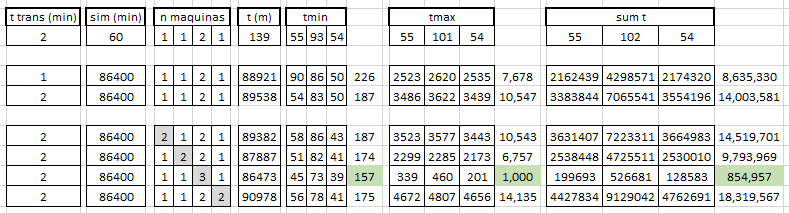
\includegraphics{./imagenes/r1.PNG}
\caption{r1.png}
\end{figure}

    \begin{figure}
\centering
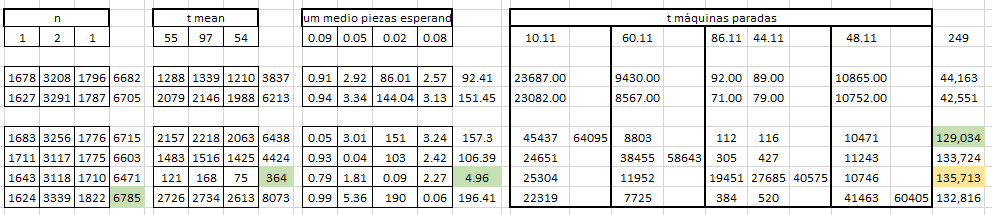
\includegraphics{./imagenes/r2.PNG}
\caption{r2.png}
\end{figure}

    Podemos leer de los resultados que se muestran en las imágenes
anteriores que el Caso3, en el que se añade una tercera máquina a la
célula 3, es el que resulta más favorable al analizar todas las métricas
(marcado en verde los resultados mejores)

Si analizamos concretamente estos resultados vemos que la agregación de
tiempos (máximos, mínimos y suma) de la fabricación para las 3 piezas
dan resultados muy inferiores al resto de casos y que destaca
fundamentalmente en la suma de tiempos de procesamiento de todas las
piezas independientemente del tipo.

Aunque el número mayor de piezas fabricadas corresponde al Caso4, si
comparamos la diferencia entre número de piezas y tiempo total empleado
en fabricarlas para los Caso3 y Caso4, resulta mucho más óptima el
comportamiento en el Caso4 ya que el tiempo necesario empleado en el
caso 4 es 20 veces superior al del Caso3 para sólo un incremento del 5\%
en la producción de las piezas.

El resultado para el promedio de tiempo de espera de las piezas es
también muy inferior en el Caso3 respecto al resto mientras el tiempo
total que están paradas las máquinas es el mayor, siendo este aspecto en
el que tiene un comportamiento menos óptimo en Caso3.


    % Add a bibliography block to the postdoc
    
    
    
    \end{document}
